\documentclass[10pt, a4paper, english]{article}\usepackage[]{graphicx}\usepackage[dvipsnames]{xcolor}
% maxwidth is the original width if it is less than linewidth
% otherwise use linewidth (to make sure the graphics do not exceed the margin)
\makeatletter
\def\maxwidth{ %
  \ifdim\Gin@nat@width>\linewidth
    \linewidth
  \else
    \Gin@nat@width
  \fi
}
\makeatother

\definecolor{fgcolor}{rgb}{0.345, 0.345, 0.345}
\newcommand{\hlnum}[1]{\textcolor[rgb]{0.686,0.059,0.569}{#1}}%
\newcommand{\hlstr}[1]{\textcolor[rgb]{0.192,0.494,0.8}{#1}}%
\newcommand{\hlcom}[1]{\textcolor[rgb]{0.678,0.584,0.686}{\textit{#1}}}%
\newcommand{\hlopt}[1]{\textcolor[rgb]{0,0,0}{#1}}%
\newcommand{\hlstd}[1]{\textcolor[rgb]{0.345,0.345,0.345}{#1}}%
\newcommand{\hlkwa}[1]{\textcolor[rgb]{0.161,0.373,0.58}{\textbf{#1}}}%
\newcommand{\hlkwb}[1]{\textcolor[rgb]{0.69,0.353,0.396}{#1}}%
\newcommand{\hlkwc}[1]{\textcolor[rgb]{0.333,0.667,0.333}{#1}}%
\newcommand{\hlkwd}[1]{\textcolor[rgb]{0.737,0.353,0.396}{\textbf{#1}}}%
\let\hlipl\hlkwb

\usepackage{framed}
\makeatletter
\newenvironment{kframe}{%
 \def\at@end@of@kframe{}%
 \ifinner\ifhmode%
  \def\at@end@of@kframe{\end{minipage}}%
  \begin{minipage}{\columnwidth}%
 \fi\fi%
 \def\FrameCommand##1{\hskip\@totalleftmargin \hskip-\fboxsep
 \colorbox{shadecolor}{##1}\hskip-\fboxsep
     % There is no \\@totalrightmargin, so:
     \hskip-\linewidth \hskip-\@totalleftmargin \hskip\columnwidth}%
 \MakeFramed {\advance\hsize-\width
   \@totalleftmargin\z@ \linewidth\hsize
   \@setminipage}}%
 {\par\unskip\endMakeFramed%
 \at@end@of@kframe}
\makeatother

\definecolor{shadecolor}{rgb}{.97, .97, .97}
\definecolor{messagecolor}{rgb}{0, 0, 0}
\definecolor{warningcolor}{rgb}{1, 0, 1}
\definecolor{errorcolor}{rgb}{1, 0, 0}
\newenvironment{knitrout}{}{} % an empty environment to be redefined in TeX

\usepackage{alltt}
%typesetting
\usepackage[margin = 1in]{geometry} % margins
\usepackage[T1]{fontenc} % font encoding
\usepackage{babel} %enables typesetting for multiple languages
\usepackage{parskip} %new lines
\usepackage{graphicx} 
\usepackage{float}
\floatplacement{figure}{H} %when printing tables, include  table.position="H"
\usepackage{bm}
\usepackage{amsmath}

\usepackage[dvipsnames]{xcolor} % more colors

\usepackage[colorlinks]{hyperref}


 %clickable table of contents from hyperref
\hypersetup{
    colorlinks,
    citecolor=black,
    filecolor=black,
    linkcolor=black,
    urlcolor=black
}

\usepackage[colorinlistoftodos]{todonotes}

\title{Machine Learning 2ST129 26605 HT2023
 Assignment 6}
\author{Anonymous Student}
\date{\today}
\IfFileExists{upquote.sty}{\usepackage{upquote}}{}
\begin{document}
\maketitle
\newpage
\tableofcontents
\newpage

\section*{General Information}
\begin{itemize}
\item Time used for reading: 3 hours 
\item Time used for basic assignment: 18 hours
\item Time used for extra assignment: 10 hours
\item Good with lab: It was good that generally for the different methods that the functions were implemented as separate function and then combined in the end, which makes it easier to understand whats going on. 
\item Things to improve with lab: I think in general there were too many questions to answer, although most of them were relatively simple it just felt that some of the things did not really connect and I just did some of them without really reflecting about them . Maybe less but more difficult questions would have been better. 
\end{itemize}
\newpage




\begin{knitrout}
\definecolor{shadecolor}{rgb}{0.969, 0.969, 0.969}\color{fgcolor}\begin{kframe}
\begin{alltt}
\hlcom{#Libraries}
 \hlkwd{library}\hlstd{(tidyverse)}
 \hlkwd{library}\hlstd{(xtable)}
 \hlkwd{library}\hlstd{(tensorflow)}
 \hlkwd{library}\hlstd{(keras)}
 \hlkwd{library}\hlstd{(bsda)}
\end{alltt}
\end{kframe}
\end{knitrout}

\begin{knitrout}
\definecolor{shadecolor}{rgb}{0.969, 0.969, 0.969}\color{fgcolor}\begin{kframe}
\begin{alltt}
\hlkwd{data}\hlstd{(}\hlstr{"iris"}\hlstd{)}
\hlkwd{data}\hlstd{(}\hlstr{"faithful"}\hlstd{)}
\hlkwd{library}\hlstd{(uuml)}
\hlkwd{data}\hlstd{(}\hlstr{"mixture_data"}\hlstd{)}
\end{alltt}
\end{kframe}
\end{knitrout}
\section{Task 1}
\subsection{1.1}
First we just visualize the faithful data 
\begin{knitrout}
\definecolor{shadecolor}{rgb}{0.969, 0.969, 0.969}\color{fgcolor}\begin{kframe}
\begin{alltt}
\hlkwd{plot}\hlstd{(faithful)}
\end{alltt}
\end{kframe}\begin{figure}
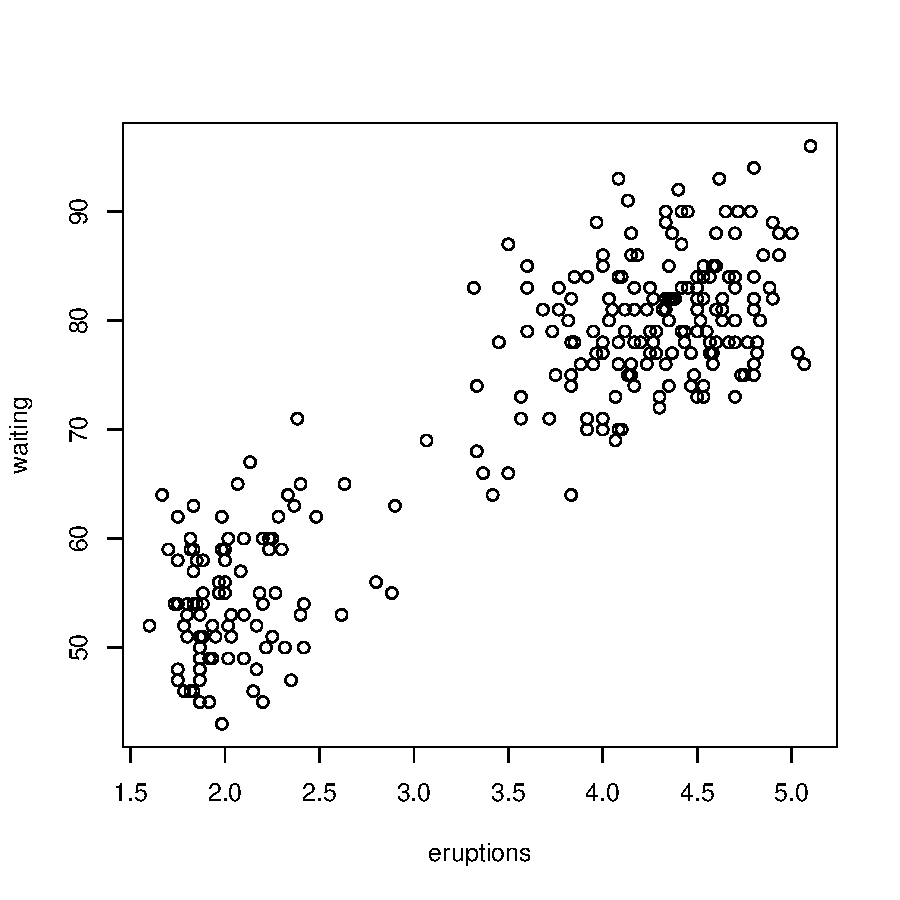
\includegraphics[width=\maxwidth]{figure/unnamed-chunk-4-1} \caption[faithful data]{faithful data}\label{fig:unnamed-chunk-4}
\end{figure}

\end{knitrout}
Visually, there seems to be two clusters that I can think of in the corners. 
\subsection{1.2}
Now we visualize the iris data set with the species as color.
\begin{knitrout}
\definecolor{shadecolor}{rgb}{0.969, 0.969, 0.969}\color{fgcolor}\begin{kframe}
\begin{alltt}
\hlstd{iris} \hlopt
  \hlkwd{ggplot}\hlstd{()} \hlopt{+}
  \hlkwd{geom_point}\hlstd{(}\hlkwd{aes}\hlstd{(}\hlkwc{x}\hlstd{=Petal.Length,} \hlkwc{y}\hlstd{= Petal.Width,} \hlkwc{color}\hlstd{=Species))}
\end{alltt}
\end{kframe}\begin{figure}
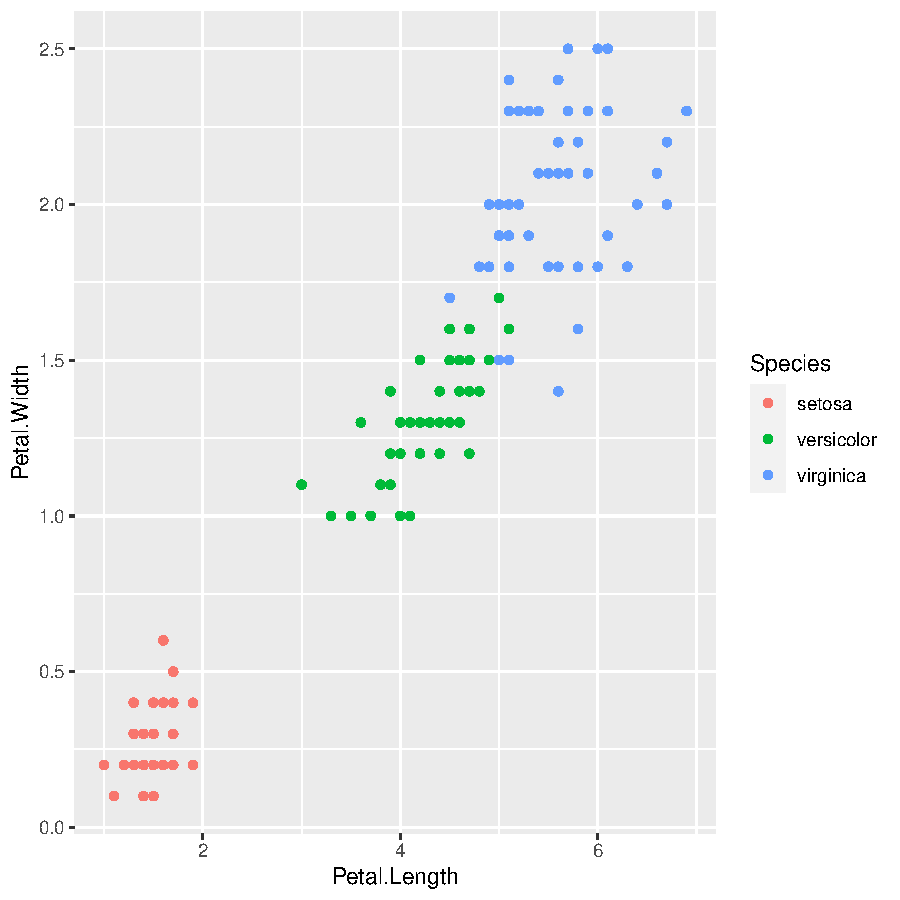
\includegraphics[width=\maxwidth]{figure/unnamed-chunk-5-1} \caption[iris data]{iris data}\label{fig:unnamed-chunk-5}
\end{figure}

\end{knitrout}

\subsection{1.3}
Now we visualize the faithful data again with the hypothesized clusters as colors. Here i based on on eruptions $<=3$
\begin{knitrout}
\definecolor{shadecolor}{rgb}{0.969, 0.969, 0.969}\color{fgcolor}\begin{kframe}
\begin{alltt}
\hlstd{index} \hlkwb{<-} \hlstd{faithful}\hlopt{$}\hlstd{eruptions} \hlopt{<=} \hlnum{3}
\hlkwd{plot}\hlstd{(faithful)}
\hlkwd{points}\hlstd{(faithful}\hlopt{$}\hlstd{eruptions[index], faithful}\hlopt{$}\hlstd{waiting[index],} \hlkwc{col}\hlstd{=}\hlstr{"red"}\hlstd{)}
\hlkwd{points}\hlstd{(faithful}\hlopt{$}\hlstd{eruptions[}\hlopt{!}\hlstd{index], faithful}\hlopt{$}\hlstd{waiting[}\hlopt{!}\hlstd{index],} \hlkwc{col}\hlstd{=}\hlstr{"blue"}\hlstd{)}
\end{alltt}
\end{kframe}\begin{figure}
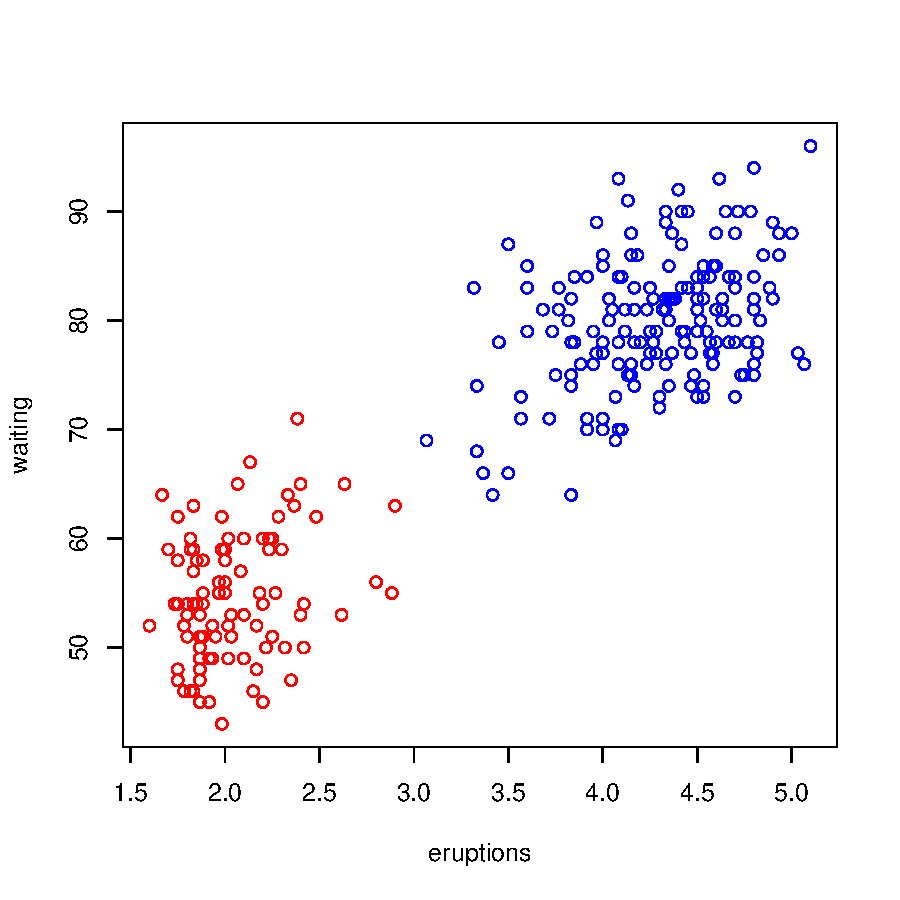
\includegraphics[width=\maxwidth]{figure/unnamed-chunk-6-1} \caption[Hypothesized clusters for eruptions]{Hypothesized clusters for eruptions}\label{fig:unnamed-chunk-6}
\end{figure}

\end{knitrout}

\subsection{1.4 } 
Now to implement the different parts of the k-means algorithm. First step 1.

\begin{knitrout}
\definecolor{shadecolor}{rgb}{0.969, 0.969, 0.969}\color{fgcolor}\begin{kframe}
\begin{alltt}
\hlcom{#' @param X n X p matrix}
\hlcom{#' @param c p x 1 vector of cluster assignments}
\hlcom{#' n is the number of rows, p is the number of cols}
\hlstd{compute_cluster_means} \hlkwb{<-} \hlkwa{function}\hlstd{(}\hlkwc{X}\hlstd{,} \hlkwc{C}\hlstd{) \{}
  \hlstd{means} \hlkwb{<-} \hlkwd{t}\hlstd{(}\hlkwd{sapply}\hlstd{(}\hlkwd{sort}\hlstd{(}\hlkwd{unique}\hlstd{(C)),} \hlkwc{FUN} \hlstd{=} \hlkwa{function}\hlstd{(}\hlkwc{i}\hlstd{)\{}
   \hlstd{index} \hlkwb{<-} \hlkwd{which}\hlstd{(C} \hlopt{==} \hlstd{i)}
   \hlkwd{colMeans}\hlstd{(X[index,])}
\hlstd{\}))}
\hlkwd{colnames}\hlstd{(means)} \hlkwb{<-} \hlkwd{colnames}\hlstd{(X)}
\hlkwd{return}\hlstd{(means)}
\hlstd{\}}

\hlkwd{set.seed}\hlstd{(}\hlnum{4711}\hlstd{)}
\hlstd{X} \hlkwb{<-} \hlkwd{as.matrix}\hlstd{(faithful)}
\hlstd{C} \hlkwb{<-} \hlkwd{sample}\hlstd{(}\hlnum{1}\hlopt{:} \hlnum{3}\hlstd{,} \hlkwd{nrow}\hlstd{(X),} \hlkwc{replace} \hlstd{=} \hlnum{TRUE}\hlstd{)}
\hlstd{m} \hlkwb{<-} \hlkwd{compute_cluster_means}\hlstd{(X,C)}
\hlstd{m}
\end{alltt}
\begin{verbatim}
     eruptions  waiting
[1,]  3.416354 70.57576
[2,]  3.571106 71.44706
[3,]  3.487659 70.72727
\end{verbatim}
\end{kframe}
\end{knitrout}


\subsection{1.5}
Now to implement the second step.
\begin{knitrout}
\definecolor{shadecolor}{rgb}{0.969, 0.969, 0.969}\color{fgcolor}\begin{kframe}
\begin{alltt}
\hlcom{#function to computer the squared distance given cluster means for one obs}
\hlcom{#assuming the number of columns match .}
\hlstd{cluster_dist} \hlkwb{<-} \hlkwa{function}\hlstd{(}\hlkwc{x_i}\hlstd{,} \hlkwc{cluster_means}\hlstd{)\{}
  \hlstd{res} \hlkwb{<-} \hlkwd{t}\hlstd{(}\hlkwd{apply}\hlstd{(cluster_means,} \hlkwc{MARGIN}\hlstd{=}\hlnum{1}\hlstd{,} \hlkwc{FUN}\hlstd{=} \hlkwa{function}\hlstd{(}\hlkwc{row}\hlstd{)\{x_i} \hlopt{-} \hlstd{row\}))}
  \hlstd{sums} \hlkwb{<-} \hlkwd{rowSums}\hlstd{(res}\hlopt{^}\hlnum{2}\hlstd{)}
  \hlstd{min_cluster} \hlkwb{<-} \hlkwd{which.min}\hlstd{(sums)}
  \hlkwd{return}\hlstd{(min_cluster)}
\hlstd{\}}

\hlcom{#' @param X n×p (design) matrix X }
\hlcom{#' @param m  K×p matrix m with one cluster mean per row}
\hlcom{#' @return  n × 1 vector of cluster assignments}
\hlstd{compute_cluster_encoding} \hlkwb{<-} \hlkwa{function}\hlstd{(}\hlkwc{X}\hlstd{,} \hlkwc{means}\hlstd{) \{}
\hlstd{new_clusters} \hlkwb{<-} \hlkwd{sapply}\hlstd{(}\hlnum{1}\hlopt{:}\hlkwd{nrow}\hlstd{(X),} \hlkwc{FUN} \hlstd{=} \hlkwa{function}\hlstd{(}\hlkwc{i}\hlstd{)\{} \hlkwd{cluster_dist}\hlstd{(X[i,], means)\})}
\hlkwd{return}\hlstd{(new_clusters)}
\hlstd{\}}

\hlstd{C} \hlkwb{<-} \hlkwd{compute_cluster_encoding}\hlstd{(X, m)}
\hlstd{C[}\hlnum{1}\hlopt{:} \hlnum{10}\hlstd{]}
\end{alltt}
\begin{verbatim}
 [1] 2 1 2 1 2 1 2 2 1 2
\end{verbatim}
\end{kframe}
\end{knitrout}

\subsection{1.6}
Now we use the functions to implement algorithm 14.1 in Hastie et al

\begin{knitrout}
\definecolor{shadecolor}{rgb}{0.969, 0.969, 0.969}\color{fgcolor}\begin{kframe}
\begin{alltt}
\hlstd{k_means} \hlkwb{<-} \hlkwa{function}\hlstd{(}\hlkwc{X}\hlstd{,}\hlkwc{k}\hlstd{)\{}
  \hlstd{clusters} \hlkwb{<-} \hlkwd{sample}\hlstd{(}\hlnum{1}\hlopt{:}\hlstd{k,} \hlkwd{nrow}\hlstd{(X),} \hlkwc{replace}\hlstd{=}\hlnum{TRUE}\hlstd{)} \hlcom{#initialize cluster assignments}
  \hlkwa{while}\hlstd{(}\hlnum{TRUE}\hlstd{)\{}
      \hlstd{c_means} \hlkwb{<-} \hlkwd{compute_cluster_means}\hlstd{(X, clusters)}
    \hlstd{new_clusters} \hlkwb{<-} \hlkwd{compute_cluster_encoding}\hlstd{(X, c_means)}
    \hlkwa{if}\hlstd{(}\hlkwd{identical}\hlstd{(new_clusters, clusters))\{}
      \hlkwa{break}
    \hlstd{\}}
    \hlstd{clusters} \hlkwb{<-} \hlstd{new_clusters}
  \hlstd{\}}
  \hlkwd{return}\hlstd{(clusters)}
\hlstd{\}}
\end{alltt}
\end{kframe}
\end{knitrout}

\subsection{1.7}
Now to implement  function to compute the k-means withing-point scatter

\begin{knitrout}
\definecolor{shadecolor}{rgb}{0.969, 0.969, 0.969}\color{fgcolor}\begin{kframe}
\begin{alltt}
\hlkwd{set.seed}\hlstd{(}\hlnum{4711}\hlstd{)}
\hlstd{X} \hlkwb{<-} \hlkwd{as.matrix}\hlstd{(faithful)}
\hlstd{C} \hlkwb{<-} \hlkwd{sample}\hlstd{(}\hlnum{1}\hlopt{:} \hlnum{3}\hlstd{,} \hlkwd{nrow}\hlstd{(X),} \hlkwc{replace} \hlstd{=} \hlnum{TRUE}\hlstd{)}

\hlstd{k_means_W} \hlkwb{<-} \hlkwa{function}\hlstd{(}\hlkwc{X}\hlstd{,}\hlkwc{C}\hlstd{)\{}
  \hlstd{c_means} \hlkwb{<-} \hlkwd{compute_cluster_means}\hlstd{(X,C)}
   \hlstd{within_cluster_sums}\hlkwb{<-} \hlkwd{sapply}\hlstd{(}\hlnum{1}\hlopt{:}\hlkwd{nrow}\hlstd{(c_means),} \hlkwc{FUN}\hlstd{=}\hlkwa{function}\hlstd{(}\hlkwc{i}\hlstd{)\{}
    \hlstd{current_cluster_m} \hlkwb{<-} \hlstd{c_means[i, ]}
    \hlstd{index} \hlkwb{<-} \hlkwd{which}\hlstd{(C} \hlopt{==} \hlstd{i)}
    \hlstd{x_subset} \hlkwb{<-} \hlstd{X[index,]}
     \hlstd{cluster_distances} \hlkwb{<-} \hlkwd{apply}\hlstd{(x_subset,} \hlnum{1}\hlstd{,}
                                \hlkwa{function}\hlstd{(}\hlkwc{row}\hlstd{)} \hlkwd{sum}\hlstd{((row} \hlopt{-} \hlstd{current_cluster_m)}\hlopt{^}\hlnum{2}\hlstd{))}
     \hlkwd{sum}\hlstd{(cluster_distances)}
\hlstd{\})}
   \hlcom{#cluster_distances are the unweighted sums within each cluster}
   \hlcom{#hence here we weight them by the cluster size which are sorted in order}
   \hlstd{aggregated_res} \hlkwb{<-} \hlkwd{sum}\hlstd{(within_cluster_sums} \hlopt{*} \hlkwd{table}\hlstd{(C))}
   \hlkwd{return}\hlstd{(aggregated_res)}
\hlstd{\}}


\hlkwd{k_means_W}\hlstd{(X,C)}
\end{alltt}
\begin{verbatim}
[1] 4601439
\end{verbatim}
\end{kframe}
\end{knitrout}

\subsection{1.8}
Now we run it a couple of times for both faithful and iris with K=2 and k=5. 
First we just create a wrapper function that will be able to be used in a \texttt{mapply()} function. Then we first start with the faithful data
\begin{knitrout}
\definecolor{shadecolor}{rgb}{0.969, 0.969, 0.969}\color{fgcolor}\begin{kframe}
\begin{alltt}
\hlcom{#wrapper function to perform the k_means and k_means_W}
\hlcom{#disclaimer: i know usually we should not set seed inside functions, but since}
\hlcom{# the goal here is to explicitly test different seeds i put in the the function}
\hlcom{#to make it easier to test}
\hlstd{k_means_wrapper} \hlkwb{<-} \hlkwa{function}\hlstd{(}\hlkwc{seed}\hlstd{,} \hlkwc{X}\hlstd{,} \hlkwc{k} \hlstd{)\{}
  \hlkwd{set.seed}\hlstd{(seed)}
  \hlstd{result} \hlkwb{<-} \hlkwd{k_means}\hlstd{(X,k)}
  \hlstd{wps} \hlkwb{<-} \hlkwd{k_means_W}\hlstd{(X, result)}

  \hlstd{list} \hlkwb{<-} \hlkwd{list}\hlstd{(}\hlstr{"Clusters"} \hlstd{= result,} \hlstr{"WPS"} \hlstd{= wps)}
  \hlkwd{return}\hlstd{(list)}

\hlstd{\}}

\hlcom{#here we use hte k_means_wrapper 10 times where the arguments are each of the }
\hlcom{# ordered pairs. So for the first 5 times we have 2 clusters and then 3 }
\hlcom{# clusters for the last 5. Each time a new seed but same X data. }

\hlstd{multi_res_faithful} \hlkwb{<-} \hlkwd{mapply}\hlstd{(}\hlkwc{FUN}\hlstd{= k_means_wrapper,}
                             \hlkwc{seed}\hlstd{=}\hlkwd{c}\hlstd{(}\hlnum{1}\hlstd{,}\hlnum{2}\hlstd{,}\hlnum{3}\hlstd{,}\hlnum{4}\hlstd{,}\hlnum{5}\hlstd{,}\hlnum{6}\hlstd{,}\hlnum{7}\hlstd{,}\hlnum{8}\hlstd{,}\hlnum{9}\hlstd{,}\hlnum{10}\hlstd{),} \hlkwc{X}\hlstd{=}\hlkwd{list}\hlstd{(X),}
                            \hlkwc{k}\hlstd{=}\hlkwd{c}\hlstd{(}\hlkwd{rep}\hlstd{(}\hlnum{2}\hlstd{,}\hlnum{5}\hlstd{),} \hlkwd{rep}\hlstd{(}\hlnum{3}\hlstd{,}\hlnum{5}\hlstd{)),} \hlkwc{SIMPLIFY} \hlstd{=} \hlnum{FALSE}\hlstd{)}
\hlstd{merged_res} \hlkwb{<-} \hlkwd{do.call}\hlstd{(rbind, multi_res_faithful)}

\hlstd{merged_res}
\end{alltt}
\begin{verbatim}
      Clusters    WPS     
 [1,] integer,272 1282259 
 [2,] integer,272 1282259 
 [3,] integer,272 1282259 
 [4,] integer,272 1282259 
 [5,] integer,272 1282259 
 [6,] integer,272 543213  
 [7,] integer,272 532868.4
 [8,] integer,272 577257.4
 [9,] integer,272 543213  
[10,] integer,272 532868.4
\end{verbatim}
\begin{alltt}
\hlcom{#the clusters column contains the cluster indexes for each obs.}

\hlkwd{which.min}\hlstd{(merged_res[,}\hlnum{2}\hlstd{])}
\end{alltt}
\begin{verbatim}
[1] 7
\end{verbatim}
\begin{alltt}
\hlkwd{which.max}\hlstd{(merged_res[,}\hlnum{2}\hlstd{])}
\end{alltt}
\begin{verbatim}
[1] 1
\end{verbatim}
\end{kframe}
\end{knitrout}
Looking at the results for WPS, then we see that the minimum WPS is for the seventh row, whereas the maximum value is the same for all the first 5 rows corresponding to the results which only used 2 clusters.

Next we do the same thing for this iris data.
\begin{knitrout}
\definecolor{shadecolor}{rgb}{0.969, 0.969, 0.969}\color{fgcolor}\begin{kframe}
\begin{alltt}
\hlstd{iris_data} \hlkwb{<-} \hlkwd{as.matrix}\hlstd{(iris[,}\hlopt{-}\hlnum{5}\hlstd{])}
\hlstd{multi_res_iris} \hlkwb{<-} \hlkwd{mapply}\hlstd{(}\hlkwc{FUN}\hlstd{= k_means_wrapper,}
                         \hlkwc{seed}\hlstd{=}\hlkwd{c}\hlstd{(}\hlnum{11}\hlstd{,}\hlnum{12}\hlstd{,}\hlnum{13}\hlstd{,}\hlnum{14}\hlstd{,}\hlnum{15}\hlstd{,}\hlnum{17}\hlstd{,}\hlnum{18}\hlstd{,}\hlnum{19}\hlstd{,}\hlnum{20}\hlstd{,}\hlnum{22}\hlstd{),}
                         \hlkwc{X}\hlstd{=}\hlkwd{list}\hlstd{(iris_data),} \hlkwc{k}\hlstd{=}\hlkwd{c}\hlstd{(}\hlkwd{rep}\hlstd{(}\hlnum{2}\hlstd{,}\hlnum{5}\hlstd{),}\hlkwd{rep}\hlstd{(}\hlnum{3}\hlstd{,}\hlnum{5}\hlstd{)),}
                         \hlkwc{SIMPLIFY} \hlstd{=} \hlnum{FALSE}\hlstd{)}

\hlstd{merged_res_iris} \hlkwb{<-} \hlkwd{do.call}\hlstd{(rbind, multi_res_iris)}
\hlstd{merged_res_iris}
\end{alltt}
\begin{verbatim}
      Clusters    WPS     
 [1,] integer,150 13521.46
 [2,] integer,150 13521.46
 [3,] integer,150 13521.46
 [4,] integer,150 13521.46
 [5,] integer,150 13521.46
 [6,] integer,150 4084.43 
 [7,] integer,150 4084.43 
 [8,] integer,150 4084.43 
 [9,] integer,150 4084.43 
[10,] integer,150 4084.43 
\end{verbatim}
\begin{alltt}
\hlcom{#the clusters column contains the cluster indexes for each obs.}

\hlkwd{which.min}\hlstd{(merged_res_iris[,}\hlnum{2}\hlstd{])}
\end{alltt}
\begin{verbatim}
[1] 6
\end{verbatim}
\begin{alltt}
\hlkwd{which.max}\hlstd{(merged_res_iris[,}\hlnum{2}\hlstd{])}
\end{alltt}
\begin{verbatim}
[1] 1
\end{verbatim}
\end{kframe}
\end{knitrout}
Looking at the results for Iris, we get the all the WPS are the sames given the same number of clusters such that all results for 2 clusters are 13521.46 whereas the results for 3 clusters are all 4084.  
\subsection{1.9}
Now we visualize the clusters corresponding to the best and worst WPS. Where they are tied I just chose one at random. 
\begin{knitrout}
\definecolor{shadecolor}{rgb}{0.969, 0.969, 0.969}\color{fgcolor}\begin{kframe}
\begin{alltt}
\hlstd{plot_func} \hlkwb{<-} \hlkwa{function}\hlstd{(}\hlkwc{X}\hlstd{,} \hlkwc{clusters}\hlstd{,} \hlkwc{var1}\hlstd{,} \hlkwc{var2}\hlstd{)\{}
  \hlstd{df} \hlkwb{<-} \hlkwd{cbind}\hlstd{(X,} \hlstr{"clusters"}\hlstd{= clusters)} \hlopt
    \hlkwd{as.data.frame}\hlstd{()}
  \hlstd{df}\hlopt{$}\hlstd{clusters} \hlkwb{<-} \hlkwd{as.factor}\hlstd{(df}\hlopt{$}\hlstd{clusters)}
  \hlstd{x} \hlkwb{<-} \hlkwd{ensym}\hlstd{(var1)}
  \hlstd{y} \hlkwb{=} \hlkwd{ensym}\hlstd{(var2)}
  \hlkwd{ggplot}\hlstd{(df )} \hlopt{+}
    \hlkwd{geom_point}\hlstd{(}\hlkwd{aes}\hlstd{(}\hlkwc{x}\hlstd{=}\hlopt{!!}\hlstd{x,} \hlkwc{y}\hlstd{=} \hlopt{!!}\hlstd{y,} \hlkwc{color}\hlstd{=clusters))}
  \hlcom{# "!!" is for injecting the variables from strings with ensym}
\hlstd{\}}
\end{alltt}
\end{kframe}
\end{knitrout}

\begin{knitrout}
\definecolor{shadecolor}{rgb}{0.969, 0.969, 0.969}\color{fgcolor}\begin{kframe}
\begin{alltt}
\hlcom{#here we are sapplying over the indexes corresponding to best and worse WPS}
\hlstd{plots_eruptions} \hlkwb{<-} \hlkwd{sapply}\hlstd{(}\hlkwd{c}\hlstd{(}\hlnum{1}\hlstd{,}\hlnum{7}\hlstd{),} \hlkwc{FUN} \hlstd{=} \hlkwa{function}\hlstd{(}\hlkwc{i}\hlstd{)\{}\hlkwd{plot_func}\hlstd{(X,}
                                              \hlstd{multi_res_faithful[[i]]}\hlopt{$}\hlstd{Clusters,}
  \hlkwc{var1}\hlstd{=}\hlstr{"eruptions"}\hlstd{,} \hlkwc{var2}\hlstd{=}\hlstr{"waiting"}\hlstd{)\},} \hlkwc{simplify} \hlstd{=} \hlnum{FALSE}\hlstd{)}
\hlstd{gridExtra}\hlopt{::}\hlkwd{grid.arrange}\hlstd{(plots_eruptions[[}\hlnum{1}\hlstd{]], plots_eruptions[[}\hlnum{2}\hlstd{]])}
\end{alltt}
\end{kframe}\begin{figure}
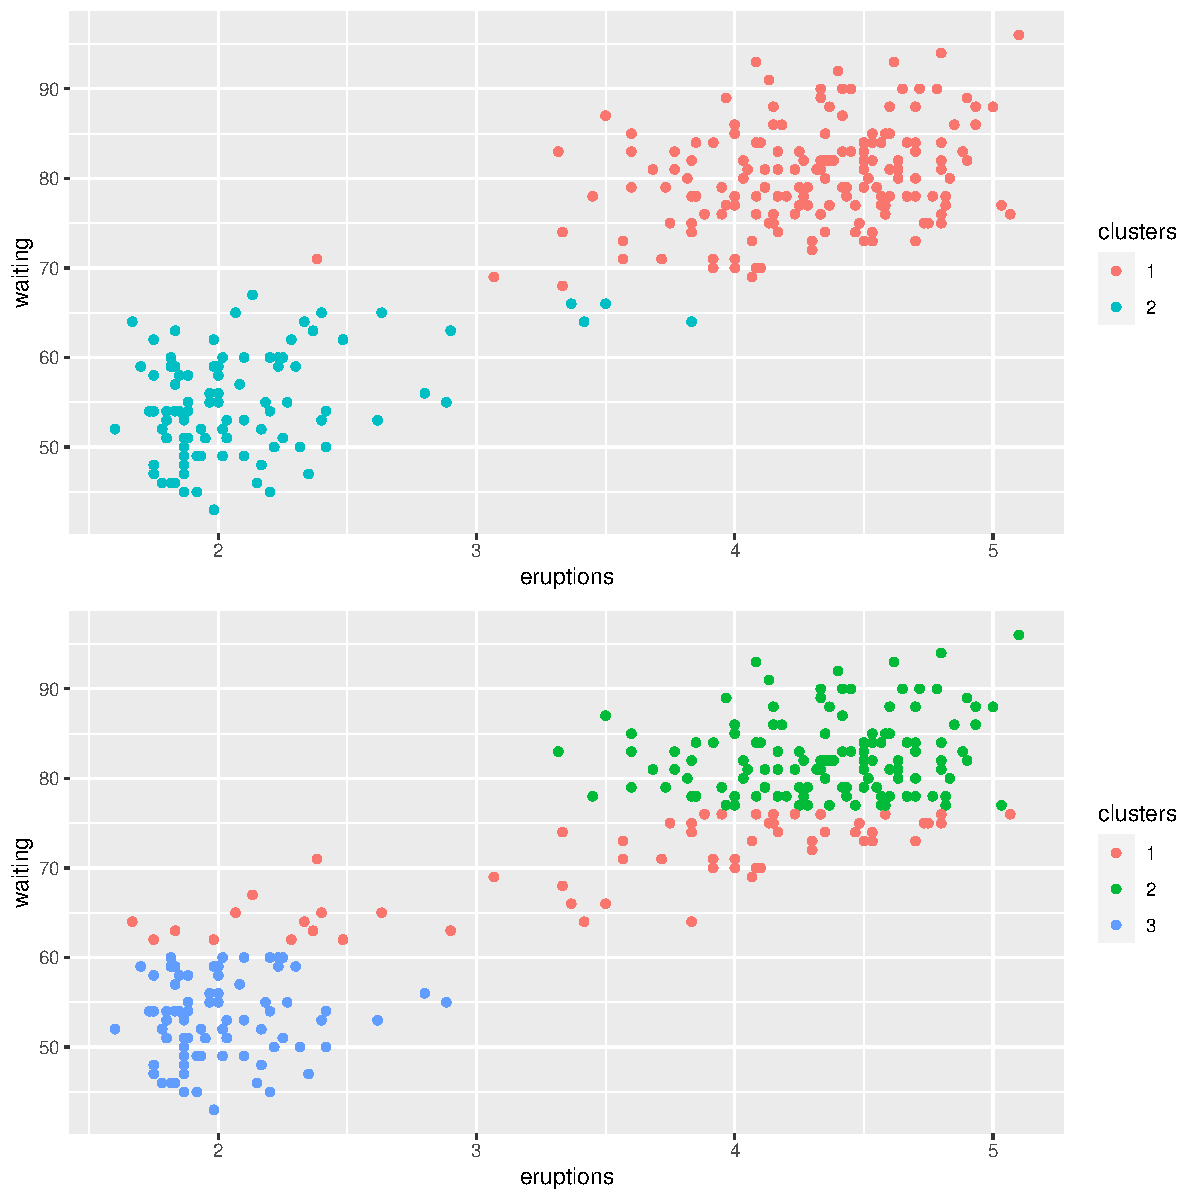
\includegraphics[width=\maxwidth]{figure/eruption_clusters-1} \caption[Clusters for eruption]{Clusters for eruption}\label{fig:eruption_clusters}
\end{figure}

\end{knitrout}


\begin{knitrout}
\definecolor{shadecolor}{rgb}{0.969, 0.969, 0.969}\color{fgcolor}\begin{kframe}
\begin{alltt}
\hlstd{plots_iris} \hlkwb{<-} \hlkwd{sapply}\hlstd{(}\hlkwd{c}\hlstd{(}\hlnum{6}\hlstd{,}\hlnum{1}\hlstd{),} \hlkwc{FUN} \hlstd{=} \hlkwa{function}\hlstd{(}\hlkwc{i}\hlstd{)\{}\hlkwd{plot_func}\hlstd{(}\hlkwd{as.matrix}\hlstd{(iris),}
                                                \hlstd{multi_res_iris[[i]]}\hlopt{$}\hlstd{Clusters,}
  \hlkwc{var1}\hlstd{=}\hlstr{"Petal.Length"}\hlstd{,} \hlkwc{var2}\hlstd{=}\hlstr{"Petal.Width"}\hlstd{)\},} \hlkwc{simplify} \hlstd{=} \hlnum{FALSE}\hlstd{)}

\hlstd{gridExtra}\hlopt{::}\hlkwd{grid.arrange}\hlstd{(plots_iris[[}\hlnum{1}\hlstd{]], plots_iris[[}\hlnum{2}\hlstd{]])}
\end{alltt}
\end{kframe}\begin{figure}
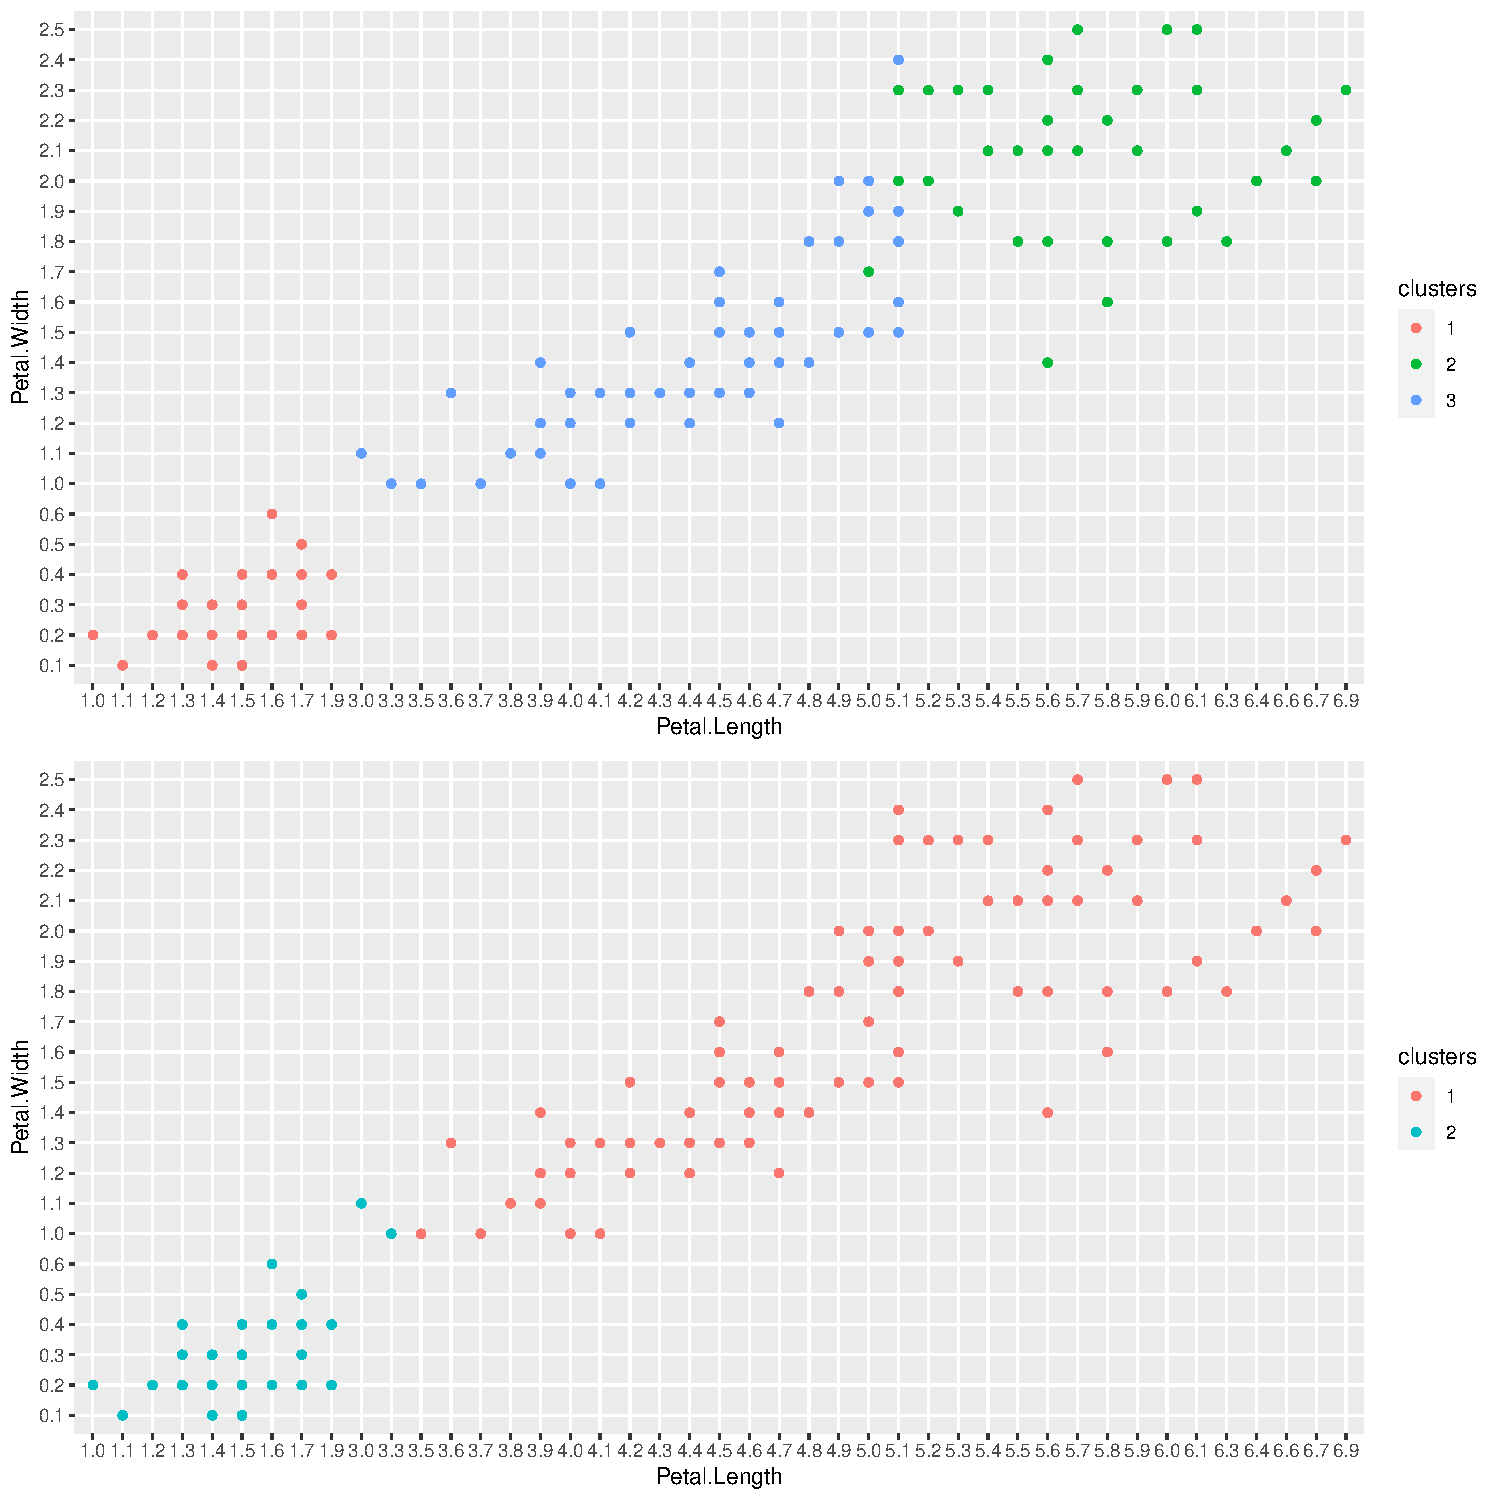
\includegraphics[width=\maxwidth]{figure/unnamed-chunk-14-1} \caption[Clusters for petal length]{Clusters for petal length}\label{fig:unnamed-chunk-14}
\end{figure}

\end{knitrout}

\subsection{1.10}

Looking at the results both from 1.8 and 1.9, then we can say that for both of the two data sets then when comparing all 10 results for the different clusters and seed, then the results seem to be similar to each other and follow a similar pattern. That is, for example in both data sets, when comparing the results for all clusters with size 2, or for all clusters with size 3, then those results given the same cluster size were similar to each other with respect to the WPS. But also that 3 clusters were always better in terms of lower WPS.

For example, for the eruption data with 2 clusters they all had the same WPS, and for 3 clusters they were not all the same but relatively similar to each other still, but when comparing 3 clusters to 2 clusters, then 3 clusters had lower WPS. 

Likewise for the iris data, the 2 cluster results had the same WPS, as well as the the 3 clusters having the same WPS. but when comparing 2 clusters to 3 clusters, than 3 clusters always had lower WPS. 


Looking at the plots of the clusters for the different data. Then we can see that for figure \ref{fig:eruption_clusters} the subplot with 2 clusters is similar to the one proposed in task 1.3, where we see two groups with, on average, one group with low values of eruptions and waiting in contrast to the other group with higher values. Looking at the plot for the one with 3 clusters, then we see that the third cluster is the one with lowest eruptions and waiting, on average. The second cluster seem to have the highest eruptions and waiting, whereas the first cluster seen ti be more spread out with regards to eruptions, but in somewhere in between the two other clusters with regard to waiting. 

As for the iris plots, we see the for the 2 cluster plot,  then one group is considerably smaller with relatively low values of petal length and petal width, whereas the other group contains a larger spread of values.  For the subplot with 3 clusters then it can bee seen that the first cluster there almost corresponds to the second cluster from the previous plot. But now we also have one cluster which is somewhere in the middle of petal length and petal width, whereas the third cluster has large values of petal length and petal width. 


\section{Task 2}
\subsection{2.1}
For this task we implement a function that simulate data from the probabilistic PCA model

We have that:
\begin{equation}
\mathbf{x} \sim \mathcal{N}\left(\boldsymbol{x} ; \boldsymbol{b}, \boldsymbol{W} \boldsymbol{W}^{\top}+\sigma^2 \boldsymbol{I}\right)
\end{equation}
or equivalently
\begin{equation}
\mathbf{x}=\boldsymbol{W} \mathbf{h}+\boldsymbol{b}+\sigma \mathbf{z}
\end{equation}

Hence we can just simulate $\bm{X}$ directly from the multivariate normal distribution.

\begin{knitrout}
\definecolor{shadecolor}{rgb}{0.969, 0.969, 0.969}\color{fgcolor}\begin{kframe}
\begin{alltt}
\hlstd{pPCA} \hlkwb{<-} \hlkwa{function}\hlstd{(}\hlkwc{W}\hlstd{,}\hlkwc{b}\hlstd{,} \hlkwc{sigma2}\hlstd{,} \hlkwc{n_sims}\hlstd{)\{}
  \hlstd{sigma2_diag} \hlkwb{<-} \hlkwd{diag}\hlstd{(}\hlkwd{length}\hlstd{(W))} \hlcom{#creating a diagonal matrix}
  \hlkwd{diag}\hlstd{(sigma2_diag)} \hlkwb{<-} \hlstd{sigma2} \hlcom{#replacing diagonals with sigma2 }
\hlstd{mv_sigma} \hlkwb{<-} \hlkwd{matrix}\hlstd{(W)} \hlopt \hlkwd{t}\hlstd{(}\hlkwd{matrix}\hlstd{(W))} \hlopt{+} \hlstd{sigma2_diag}
\hlstd{X} \hlkwb{<-} \hlkwd{rmvnorm}\hlstd{(}\hlkwc{n}\hlstd{=n_sims,} \hlkwc{mean}\hlstd{=}\hlkwd{matrix}\hlstd{(b),} \hlkwc{sigma}\hlstd{=mv_sigma )}
\hlkwd{colnames}\hlstd{(X)} \hlkwb{<-} \hlkwd{sapply}\hlstd{(}\hlnum{1}\hlopt{:}\hlkwd{ncol}\hlstd{(X),} \hlkwc{FUN} \hlstd{=} \hlkwa{function}\hlstd{(}\hlkwc{i}\hlstd{)\{} \hlkwd{paste0}\hlstd{(}\hlstr{"X"}\hlstd{,i)\})}
\hlkwd{attributes}\hlstd{(X)}\hlopt{$}\hlstd{W} \hlkwb{<-} \hlstd{W}
\hlkwd{attributes}\hlstd{(X)}\hlopt{$}\hlstd{b} \hlkwb{<-} \hlstd{b}
\hlkwd{return}\hlstd{(X)}
\hlstd{\}}
\end{alltt}
\end{kframe}
\end{knitrout}



\subsection{2.2}
Now we simulate 300 observations and plot them.
\begin{knitrout}
\definecolor{shadecolor}{rgb}{0.969, 0.969, 0.969}\color{fgcolor}\begin{kframe}
\begin{alltt}
\hlkwd{set.seed}\hlstd{(}\hlnum{1337}\hlstd{)}
\hlstd{W} \hlkwb{<-} \hlkwd{c}\hlstd{(}\hlopt{-}\hlnum{1}\hlstd{,}\hlnum{3}\hlstd{)}
\hlstd{b} \hlkwb{<-} \hlkwd{c}\hlstd{(}\hlnum{0.5}\hlstd{,} \hlnum{2}\hlstd{)}
\hlstd{results} \hlkwb{<-} \hlkwd{pPCA}\hlstd{(W,b,}\hlkwc{sigma2}\hlstd{=}\hlnum{1}\hlstd{,}\hlkwc{n_sim}\hlstd{=}\hlnum{300}\hlstd{)}
\end{alltt}
\end{kframe}
\end{knitrout}


\begin{knitrout}
\definecolor{shadecolor}{rgb}{0.969, 0.969, 0.969}\color{fgcolor}\begin{kframe}
\begin{alltt}
\hlkwd{plot}\hlstd{(results)}
\end{alltt}
\end{kframe}\begin{figure}
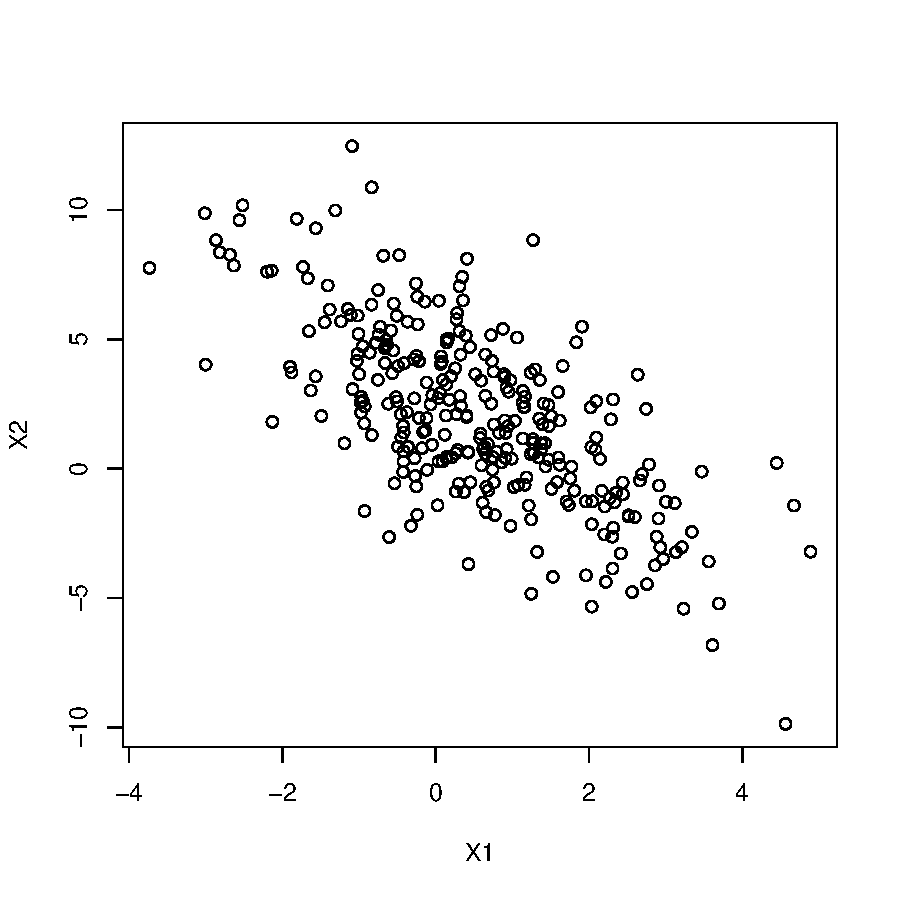
\includegraphics[width=\maxwidth]{figure/unnamed-chunk-17-1} \caption[Visualization of 300 simulated observations]{Visualization of 300 simulated observations}\label{fig:unnamed-chunk-17}
\end{figure}

\end{knitrout}

\subsection{2.3}
As described by the equation in 2.1, this model assumes that $\bm{x}$ follows a multivariate normal distribution as $$\mathbf{x} \sim \mathcal{N}\left(\boldsymbol{x} ; \boldsymbol{b}, \boldsymbol{W} \boldsymbol{W}^{\top}+\sigma^2 \boldsymbol{I}\right)$$

Hence the argument b in the code corresponds to the mean vector $\bm{b}$ and that the terms $\bm{WW}^T + \sigma^2\bm{I}$ corresponds to the variance matrix. Also we can say that the argument W corresponds to the factor loadings in the model recalling that it could also be represented on the form:
$$
\mathbf{x}=\boldsymbol{W} \mathbf{h}+\boldsymbol{b}+\sigma \mathbf{z}
$$ where $\bm{h}$ here represents the latent variables. 

\subsection{2.4}
Now we test some other parameter values for W and b and visualize the results.

\begin{knitrout}
\definecolor{shadecolor}{rgb}{0.969, 0.969, 0.969}\color{fgcolor}\begin{kframe}
\begin{alltt}
\hlstd{W_list} \hlkwb{<-} \hlkwd{list}\hlstd{(}\hlkwd{c}\hlstd{(}\hlnum{1}\hlstd{,}\hlnum{2}\hlstd{),} \hlkwd{c}\hlstd{(}\hlopt{-}\hlnum{3}\hlstd{,}\hlnum{3}\hlstd{),}
               \hlkwd{c}\hlstd{(}\hlnum{2}\hlstd{,}\hlopt{-}\hlnum{5}\hlstd{),} \hlkwd{c}\hlstd{(}\hlnum{0}\hlstd{,}\hlnum{0}\hlstd{),}
               \hlkwd{c}\hlstd{(}\hlnum{6}\hlstd{,}\hlnum{10}\hlstd{),} \hlkwd{c}\hlstd{(}\hlopt{-}\hlnum{5}\hlstd{,}\hlnum{15}\hlstd{))}

\hlstd{b_list} \hlkwb{<-} \hlkwd{list}\hlstd{(}\hlkwd{c}\hlstd{(}\hlnum{1}\hlstd{,}\hlnum{3}\hlstd{),} \hlkwd{c}\hlstd{(}\hlopt{-}\hlnum{2}\hlstd{,}\hlnum{5}\hlstd{),}
               \hlkwd{c}\hlstd{(}\hlnum{0.8}\hlstd{,} \hlnum{6}\hlstd{),} \hlkwd{c}\hlstd{(}\hlopt{-}\hlnum{1}\hlstd{,} \hlnum{1}\hlstd{),}
               \hlkwd{c}\hlstd{(}\hlnum{2}\hlstd{,} \hlopt{-}\hlnum{3}\hlstd{),} \hlkwd{c}\hlstd{(}\hlnum{10}\hlstd{,} \hlnum{3}\hlstd{))}
\hlkwd{set.seed}\hlstd{(}\hlnum{1337}\hlstd{)}
\hlstd{multi_res} \hlkwb{<-} \hlkwd{mapply}\hlstd{(}\hlkwc{FUN}\hlstd{=pPCA,} \hlkwc{W}\hlstd{=W_list,} \hlkwc{b}\hlstd{=b_list,} \hlkwc{n_sims}\hlstd{=}\hlnum{300}\hlstd{,} \hlkwc{sigma2}\hlstd{=}\hlnum{1}\hlstd{,} \hlkwc{SIMPLIFY} \hlstd{=} \hlnum{FALSE}\hlstd{)}
\end{alltt}
\end{kframe}
\end{knitrout}

\begin{knitrout}
\definecolor{shadecolor}{rgb}{0.969, 0.969, 0.969}\color{fgcolor}\begin{kframe}
\begin{alltt}
\hlkwd{par}\hlstd{(}\hlkwc{mfrow}\hlstd{=}\hlkwd{c}\hlstd{(}\hlnum{2}\hlstd{,}\hlnum{3}\hlstd{))}
\hlkwd{lapply}\hlstd{(multi_res,} \hlkwc{FUN} \hlstd{=} \hlkwa{function}\hlstd{(}\hlkwc{i}\hlstd{)\{}
  \hlstd{W} \hlkwb{<-} \hlkwd{attributes}\hlstd{(i)}\hlopt{$}\hlstd{W}
  \hlstd{b} \hlkwb{<-} \hlkwd{attributes}\hlstd{(i)}\hlopt{$}\hlstd{b}
\hlstd{main} \hlkwb{<-} \hlkwd{paste}\hlstd{(}\hlstr{"W = ("}\hlstd{,} \hlkwd{paste}\hlstd{(W,} \hlkwc{collapse} \hlstd{=} \hlstr{", "}\hlstd{),} \hlstr{")"}\hlstd{,} \hlstr{", "}\hlstd{,}
              \hlstr{"b = ("}\hlstd{,} \hlkwd{paste}\hlstd{(b,} \hlkwc{collapse} \hlstd{=} \hlstr{", "}\hlstd{),} \hlstr{")"} \hlstd{)}
  \hlkwd{plot}\hlstd{(i,} \hlkwc{main}\hlstd{=main)}
\hlstd{\})}
\end{alltt}
\end{kframe}\begin{figure}
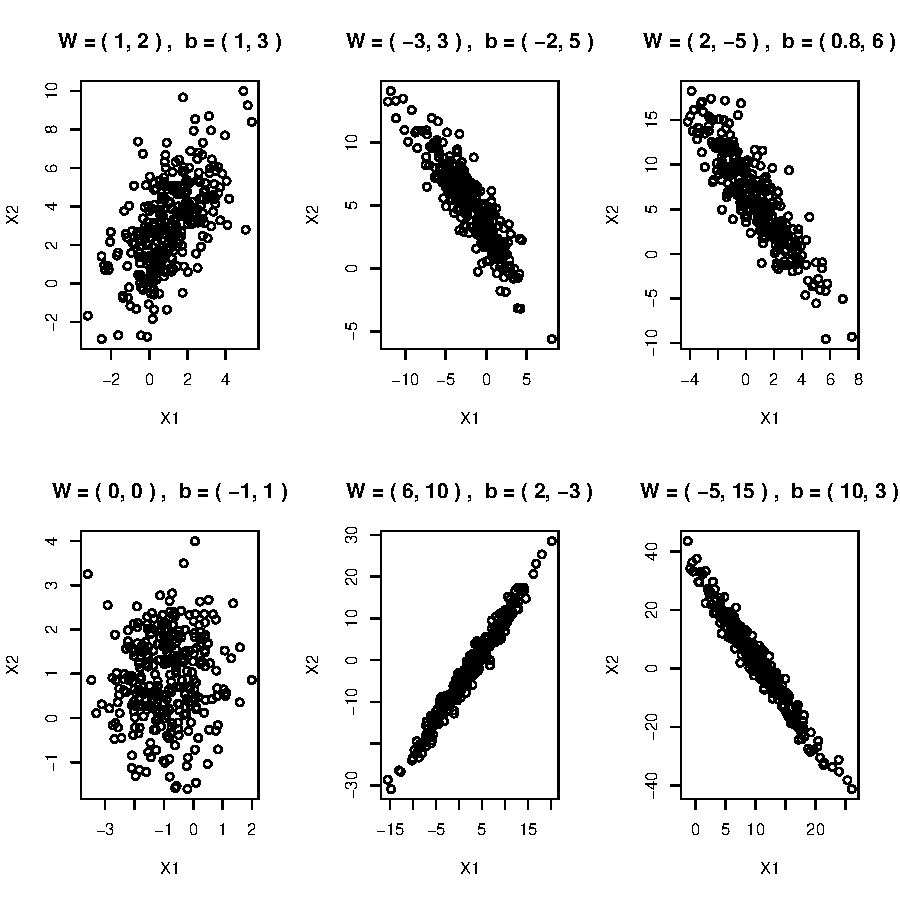
\includegraphics[width=\maxwidth]{figure/unnamed-chunk-19-1} \caption[Results for different values of W and b]{Results for different values of W and b}\label{fig:unnamed-chunk-19}
\end{figure}

\begin{kframe}\begin{alltt}
\hlkwd{par}\hlstd{(}\hlkwc{mfrow}\hlstd{=}\hlkwd{c}\hlstd{(}\hlnum{1}\hlstd{,}\hlnum{1}\hlstd{))}
\end{alltt}
\end{kframe}
\end{knitrout}

\subsection{2.5} 
Now we run PCA on the simulated data from task 2.2.
\begin{knitrout}
\definecolor{shadecolor}{rgb}{0.969, 0.969, 0.969}\color{fgcolor}\begin{kframe}
\begin{alltt}
\hlstd{pr_res} \hlkwb{<-} \hlkwd{prcomp}\hlstd{(results,} \hlkwc{center}\hlstd{=}\hlnum{TRUE}\hlstd{,} \hlkwc{scale}\hlstd{=} \hlnum{FALSE}\hlstd{)}
\hlstd{pr_res}\hlopt{$}\hlstd{rotation[,}\hlnum{1}\hlstd{]} \hlopt{*} \hlstd{pr_res}\hlopt{$}\hlstd{sdev[}\hlnum{1}\hlstd{]} \hlopt{* -}\hlnum{1}
\end{alltt}
\begin{verbatim}
       X1        X2 
-1.107786  3.414624 
\end{verbatim}
\end{kframe}
\end{knitrout}

\subsection{2.6}
Looking at the results, it can be seen that this corresponds to the parameters in $\bm{W}$, seeing as they are close but not exactly the same .

\subsection{2.7}

For this task we want to simulate new data $\bm{x}$ with five dimensions. We can do that by reusing the previously defined function but increasing the dimension for $\bm{W}$ and $\bm{b}$. I will just simulate some values for them but also make sure in the end that we get both positive and negative correlations

\begin{knitrout}
\definecolor{shadecolor}{rgb}{0.969, 0.969, 0.969}\color{fgcolor}\begin{kframe}
\begin{alltt}
\hlkwd{set.seed}\hlstd{(}\hlnum{1337}\hlstd{)}
\hlstd{new_W} \hlkwb{=} \hlkwd{sample}\hlstd{(}\hlopt{-}\hlnum{5}\hlopt{:}\hlnum{5}\hlstd{,} \hlnum{5}\hlstd{,} \hlkwc{replace}\hlstd{=}\hlnum{FALSE}\hlstd{)}
\hlstd{new_b} \hlkwb{<-} \hlkwd{sample}\hlstd{(}\hlopt{-}\hlnum{10}\hlopt{:}\hlnum{10}\hlstd{,} \hlnum{5}\hlstd{,} \hlkwc{replace}\hlstd{=}\hlnum{TRUE}\hlstd{)}
\hlkwd{print}\hlstd{(new_W)}
\end{alltt}
\begin{verbatim}
[1]  4 -3 -4 -5  3
\end{verbatim}
\begin{alltt}
\hlkwd{print}\hlstd{(new_b)}
\end{alltt}
\begin{verbatim}
[1]  8 -7 -6  3 -2
\end{verbatim}
\begin{alltt}
\hlstd{new_results}  \hlkwb{<-} \hlkwd{pPCA}\hlstd{(}\hlkwc{W} \hlstd{= new_W,} \hlkwc{b} \hlstd{= new_b,} \hlkwc{sigma2} \hlstd{=} \hlnum{1.3}\hlstd{,} \hlkwc{n}\hlstd{=}\hlnum{500}\hlstd{)}
\hlkwd{pairs}\hlstd{(new_results)}
\end{alltt}
\end{kframe}
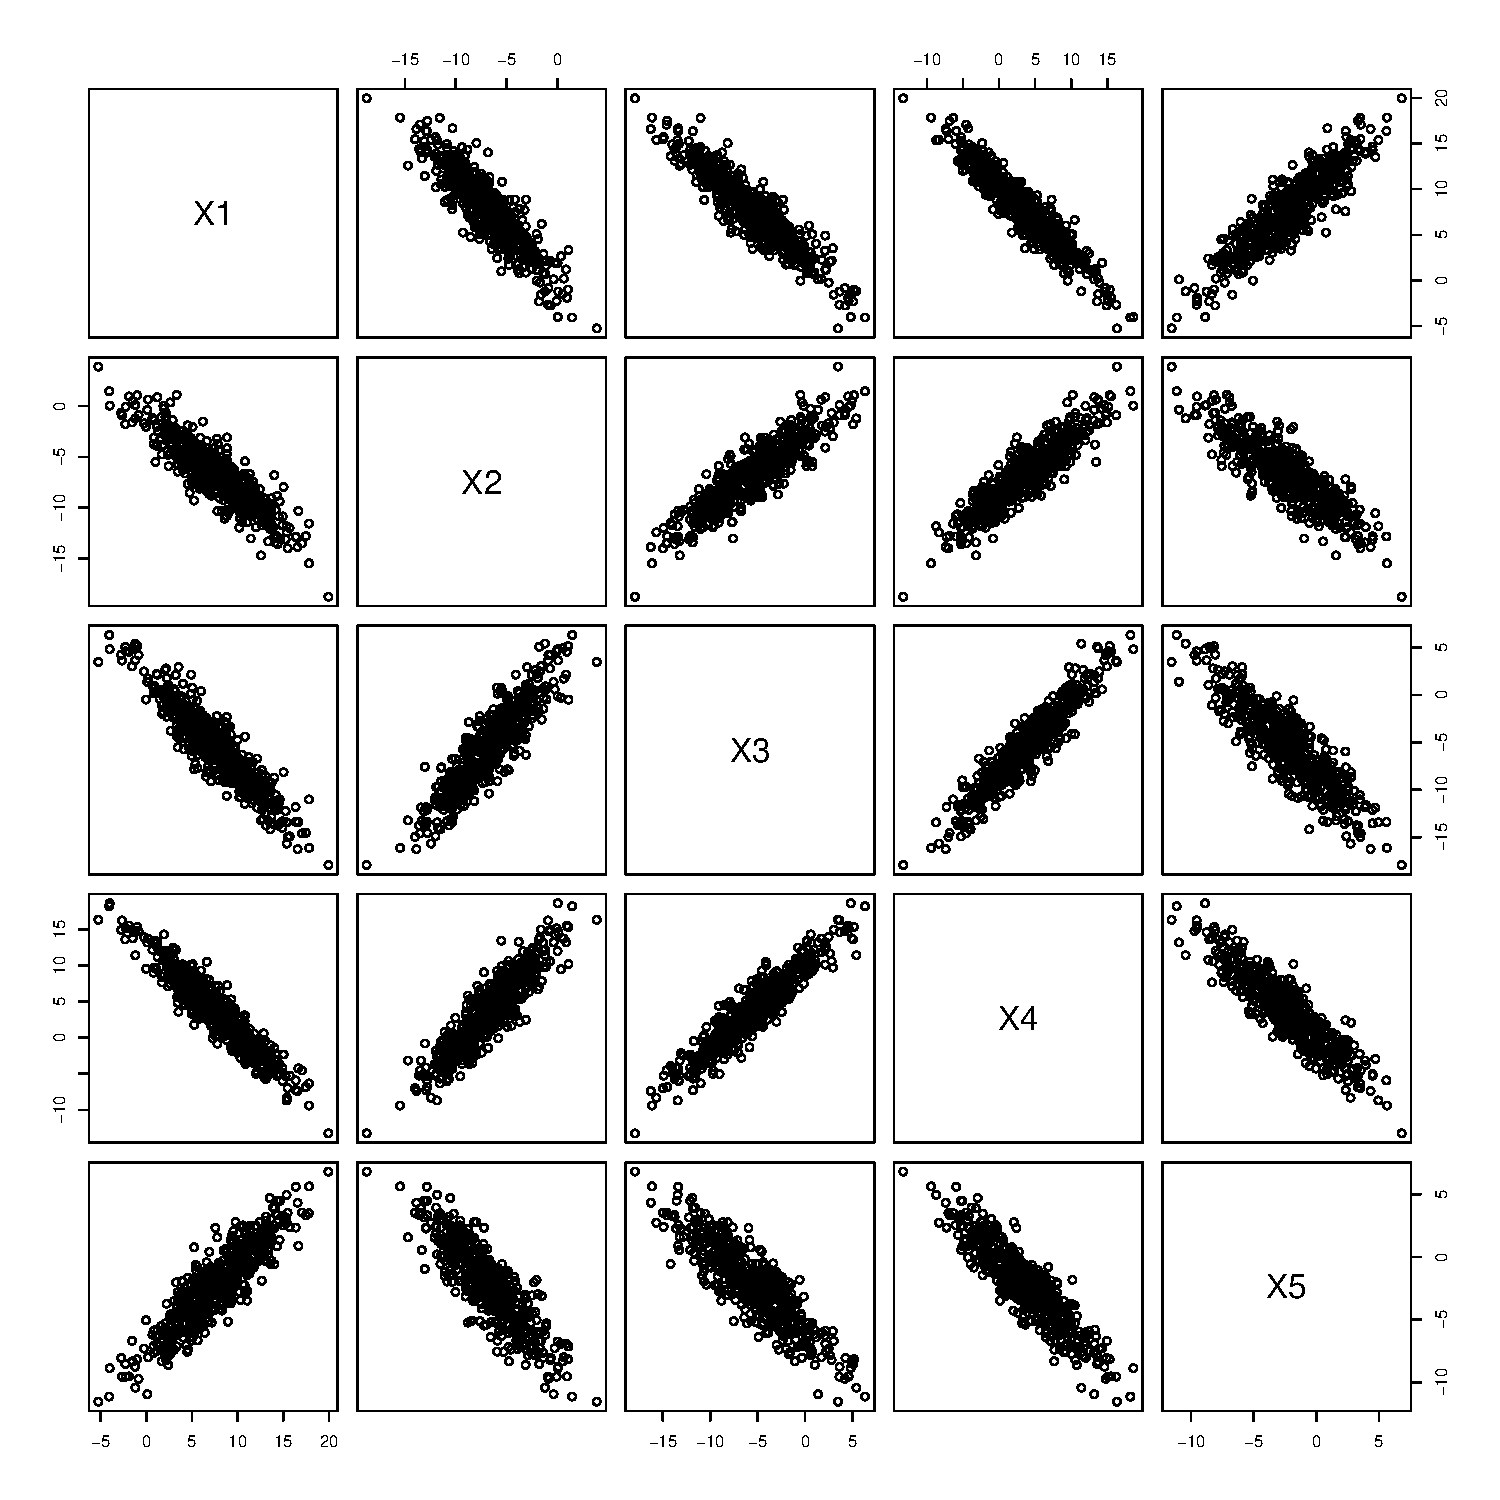
\includegraphics[width=\maxwidth]{figure/unnamed-chunk-21-1} 
\end{knitrout}
\section{Task 3}
\begin{knitrout}
\definecolor{shadecolor}{rgb}{0.969, 0.969, 0.969}\color{fgcolor}\begin{kframe}
\begin{alltt}
\hlkwd{library}\hlstd{(uuml)}
\hlkwd{data}\hlstd{(}\hlstr{"mixture_data"}\hlstd{)}
\hlstd{theta0} \hlkwb{<-} \hlkwd{list}\hlstd{(}\hlkwc{mu_1} \hlstd{=} \hlnum{4.12}\hlstd{,} \hlkwc{mu_2} \hlstd{=} \hlnum{0.94}\hlstd{,} \hlkwc{sigma_1} \hlstd{=} \hlnum{2}\hlstd{,} \hlkwc{sigma_2} \hlstd{=} \hlnum{2}\hlstd{,} \hlkwc{pi} \hlstd{=} \hlnum{0.5}\hlstd{)}
\hlstd{theta0}
\end{alltt}
\begin{verbatim}
$mu_1
[1] 4.12

$mu_2
[1] 0.94

$sigma_1
[1] 2

$sigma_2
[1] 2

$pi
[1] 0.5
\end{verbatim}
\begin{alltt}
\hlkwd{hist}\hlstd{(mixture_data)}
\end{alltt}
\end{kframe}
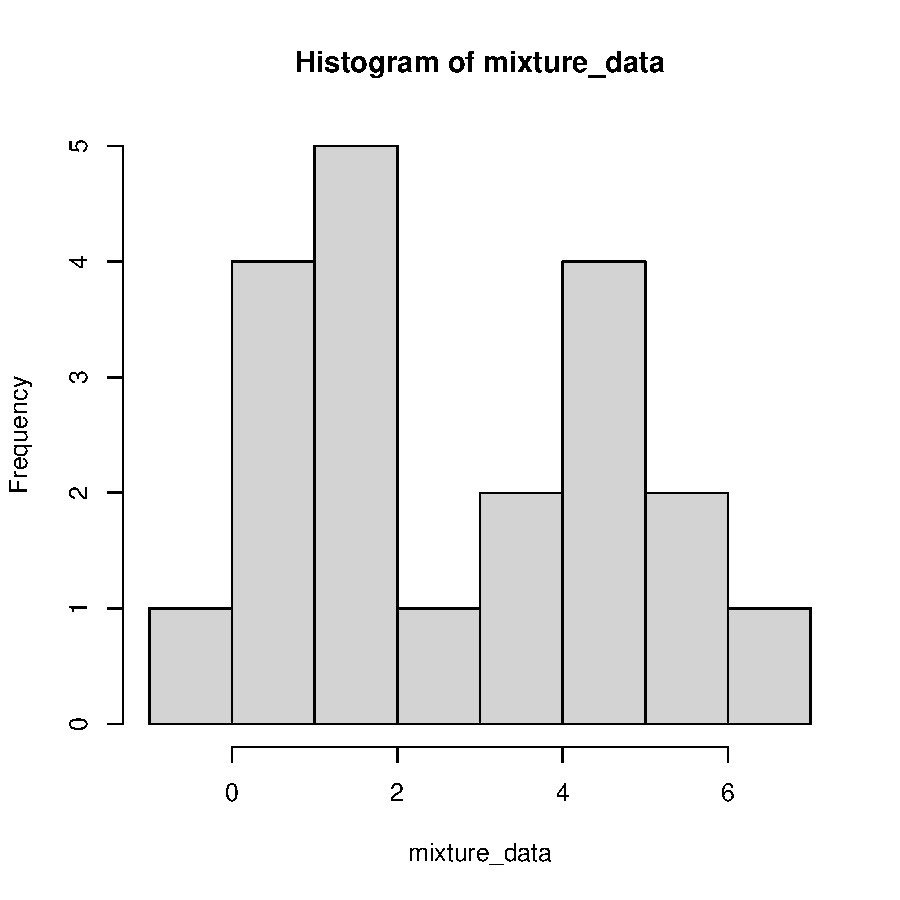
\includegraphics[width=\maxwidth]{figure/unnamed-chunk-22-1} 
\end{knitrout}


\subsection{3.1}
First we create a function to simulate data from a univariate mixture model.
\begin{knitrout}
\definecolor{shadecolor}{rgb}{0.969, 0.969, 0.969}\color{fgcolor}\begin{kframe}
\begin{alltt}
\hlstd{r_uni_two_comp}\hlkwb{<-} \hlkwa{function}\hlstd{(}\hlkwc{n}\hlstd{,} \hlkwc{theta}\hlstd{)\{}
  \hlcom{#sample delta for each obs}
  \hlstd{deltas} \hlkwb{<-} \hlkwd{rbinom}\hlstd{(}\hlkwc{n}\hlstd{=n,} \hlnum{1}\hlstd{,} \hlkwc{p}\hlstd{=theta}\hlopt{$}\hlstd{pi)}
  \hlstd{y_1} \hlkwb{<-} \hlkwd{rnorm}\hlstd{(}\hlkwc{n}\hlstd{=n,} \hlkwc{mean}\hlstd{=theta}\hlopt{$}\hlstd{mu_1,} \hlkwc{sd}\hlstd{= theta}\hlopt{$}\hlstd{sigma_1)}
  \hlstd{y_2} \hlkwb{<-} \hlkwd{rnorm}\hlstd{(}\hlkwc{n}\hlstd{=n,} \hlkwc{mean}\hlstd{=theta}\hlopt{$}\hlstd{mu_2,} \hlkwc{sd}\hlstd{=theta}\hlopt{$}\hlstd{sigma_2)}
  \hlstd{Y} \hlkwb{<-} \hlstd{(}\hlnum{1}\hlopt{-}\hlstd{deltas)} \hlopt{*} \hlstd{y_1} \hlopt{+} \hlstd{deltas}\hlopt{*}\hlstd{y_2}
  \hlkwd{return}\hlstd{(Y)}
  \hlcom{#samply y_i from the relevant component}
\hlstd{\}}
\hlkwd{head}\hlstd{(}\hlkwd{r_uni_two_comp}\hlstd{(}\hlkwc{n}\hlstd{=}\hlnum{100}\hlstd{,} \hlkwc{theta}\hlstd{=theta0))}
\end{alltt}
\begin{verbatim}
[1] 2.2514313 2.9134916 4.7977395 3.1977811 2.7223639 0.3170157
\end{verbatim}
\end{kframe}
\end{knitrout}


\subsection{3.2}
Now to simulate 200 observations using $\mu_1=-2, \mu_2 = 1.5, \sigma_1 = 2, \sigma_2=1, \pi=0.3$
\begin{knitrout}
\definecolor{shadecolor}{rgb}{0.969, 0.969, 0.969}\color{fgcolor}\begin{kframe}
\begin{alltt}
\hlkwd{set.seed}\hlstd{(}\hlnum{1337}\hlstd{)}
\hlstd{thetas} \hlkwb{<-}\hlkwd{list}\hlstd{(}\hlkwc{mu_1}\hlstd{=}\hlopt{-}\hlnum{2}\hlstd{,} \hlkwc{mu_2}\hlstd{=}\hlnum{1.5}\hlstd{,}
              \hlkwc{sigma_1}\hlstd{=}\hlnum{2}\hlstd{,} \hlkwc{sigma_2}\hlstd{=}\hlnum{1}\hlstd{,}
              \hlkwc{pi}\hlstd{=}\hlnum{0.3}\hlstd{)}

\hlstd{observations} \hlkwb{<-} \hlkwd{r_uni_two_comp}\hlstd{(}\hlnum{200}\hlstd{, thetas)}
\hlkwd{hist}\hlstd{(observations)}
\end{alltt}
\end{kframe}\begin{figure}
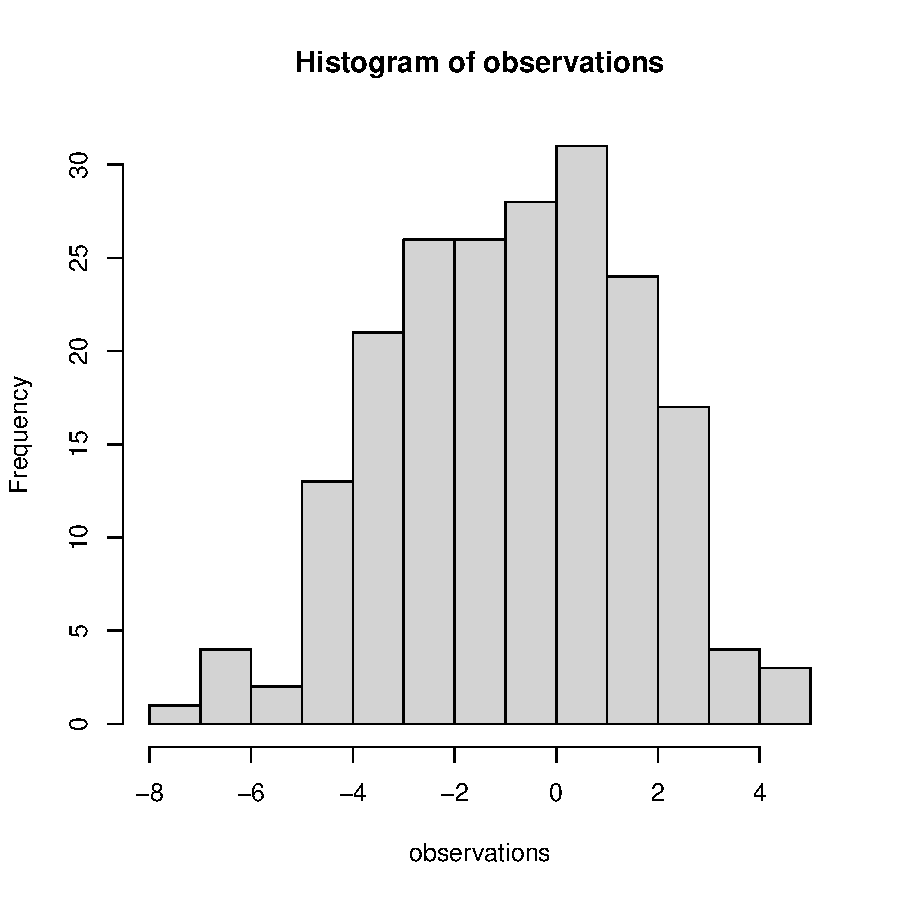
\includegraphics[width=\maxwidth]{figure/unnamed-chunk-24-1} \caption[Distribution for simulated observations]{Distribution for simulated observations}\label{fig:unnamed-chunk-24}
\end{figure}

\end{knitrout}

\subsection{3.3}
Now we implement a function to compute the density values for a given set of parameters theta for values of x.
\begin{knitrout}
\definecolor{shadecolor}{rgb}{0.969, 0.969, 0.969}\color{fgcolor}\begin{kframe}
\begin{alltt}
\hlstd{d_uni_two_comp} \hlkwb{<-} \hlkwa{function}\hlstd{(}\hlkwc{x}\hlstd{,} \hlkwc{theta}\hlstd{)\{}
  \hlstd{dens_1} \hlkwb{<-} \hlkwd{dnorm}\hlstd{(x,} \hlkwc{mean}\hlstd{=theta}\hlopt{$}\hlstd{mu_1,} \hlkwc{sd} \hlstd{= theta}\hlopt{$}\hlstd{sigma_1)}
  \hlstd{dens_2} \hlkwb{<-} \hlkwd{dnorm}\hlstd{(x,} \hlkwc{mean}\hlstd{=theta}\hlopt{$}\hlstd{mu_2,} \hlkwc{sd}\hlstd{=theta}\hlopt{$}\hlstd{sigma_2)}
  \hlstd{g_x} \hlkwb{<-} \hlstd{(}\hlnum{1}\hlopt{-}\hlstd{theta}\hlopt{$}\hlstd{pi)} \hlopt{*} \hlstd{dens_1} \hlopt{+} \hlstd{theta}\hlopt{$}\hlstd{pi}\hlopt{*}\hlstd{dens_2}
  \hlkwd{return}\hlstd{(g_x)}
\hlstd{\}}
\end{alltt}
\end{kframe}
\end{knitrout}

\subsection{3.4}
Now we visualize the density for the mixture model.
\begin{knitrout}
\definecolor{shadecolor}{rgb}{0.969, 0.969, 0.969}\color{fgcolor}\begin{kframe}
\begin{alltt}
\hlstd{plot_density} \hlkwb{<-} \hlkwa{function}\hlstd{(}\hlkwc{x}\hlstd{,} \hlkwc{theta}\hlstd{,}\hlkwc{...}\hlstd{)\{}
  \hlstd{densities} \hlkwb{<-} \hlkwd{d_uni_two_comp}\hlstd{(x, theta)}
  \hlkwd{plot}\hlstd{(}\hlkwc{x}\hlstd{=x,} \hlkwc{y}\hlstd{=densities,} \hlkwc{col}\hlstd{=}\hlstr{"blue"}\hlstd{, ...)}
\hlstd{\}}

\hlkwd{plot_density}\hlstd{(}\hlkwc{x}\hlstd{=}\hlkwd{seq}\hlstd{(}\hlopt{-}\hlnum{4}\hlstd{,}\hlnum{4}\hlstd{,} \hlkwc{by}\hlstd{=}\hlnum{0.01}\hlstd{),} \hlkwc{theta}\hlstd{=thetas)}
\end{alltt}
\end{kframe}\begin{figure}
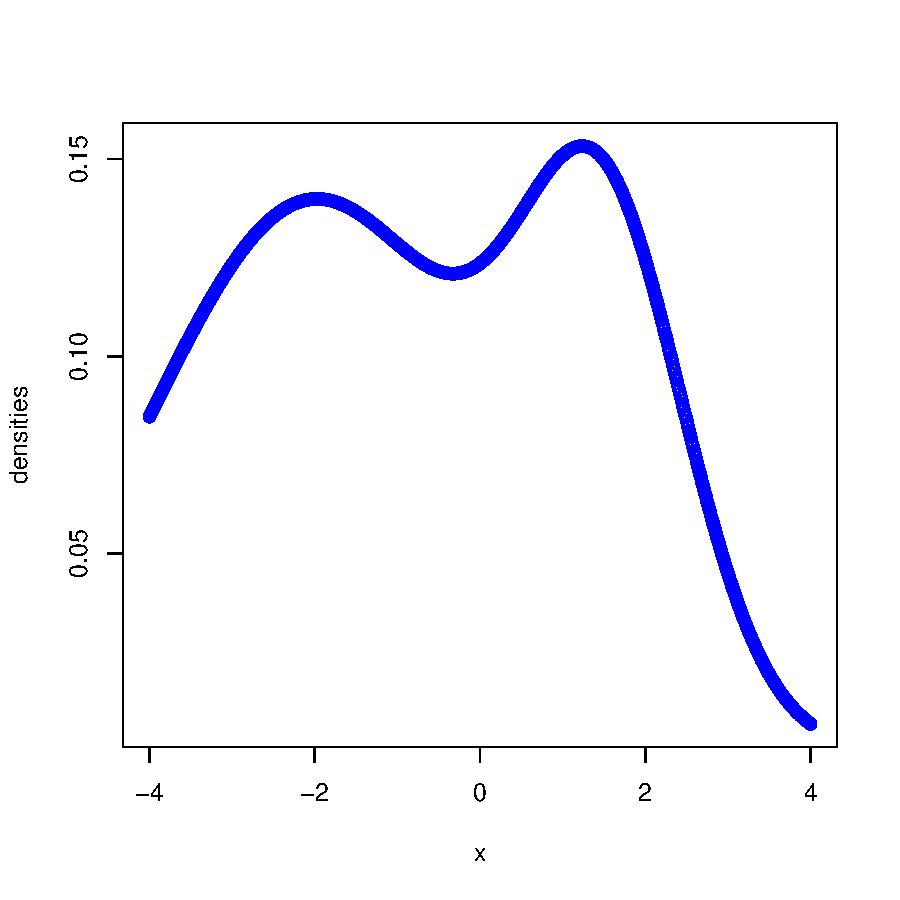
\includegraphics[width=\maxwidth]{figure/unnamed-chunk-26-1} \caption[Density for the mixture model from -4 to 4]{Density for the mixture model from -4 to 4}\label{fig:unnamed-chunk-26}
\end{figure}

\end{knitrout}

\subsection{3.5}
now we visualize the eruptions variable in the faithful data
\begin{knitrout}
\definecolor{shadecolor}{rgb}{0.969, 0.969, 0.969}\color{fgcolor}\begin{kframe}
\begin{alltt}
\hlkwd{hist}\hlstd{(faithful}\hlopt{$}\hlstd{eruptions)}
\end{alltt}
\end{kframe}\begin{figure}
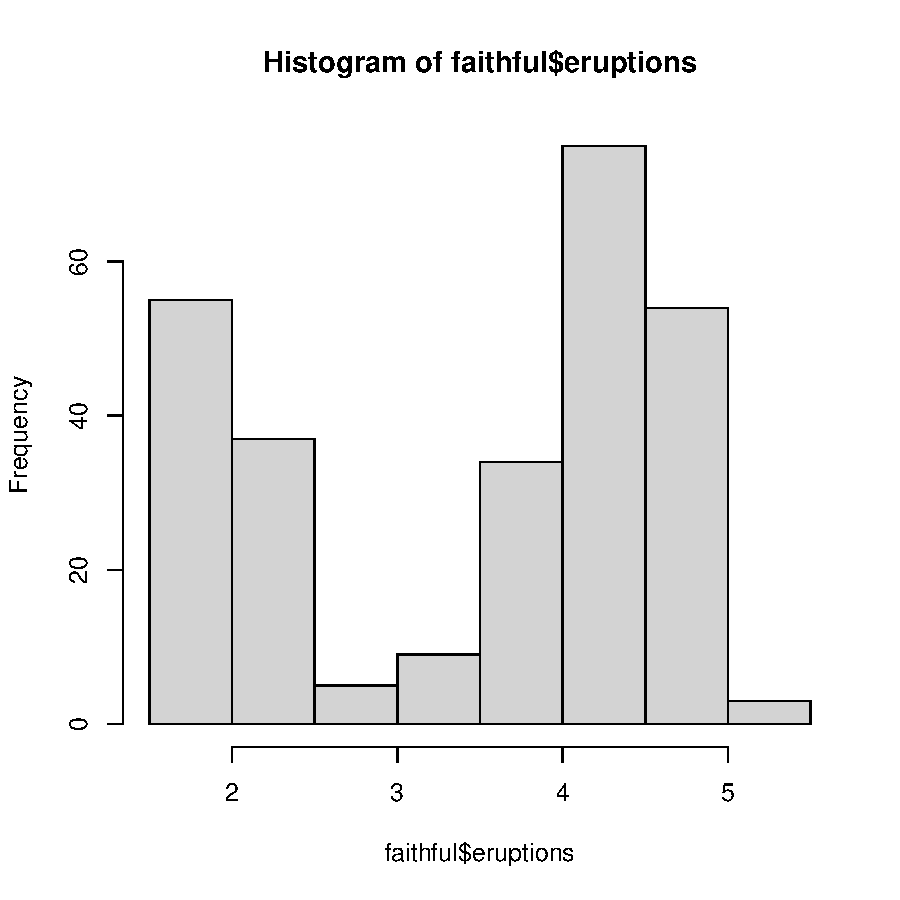
\includegraphics[width=\maxwidth]{figure/eruptions-1} \caption[Distribution of eruptions]{Distribution of eruptions}\label{fig:eruptions}
\end{figure}

\end{knitrout}



\subsection{3.6}
Based on the figure \ref{fig:eruptions} we see that there are two peaks. One around 2 and one around 4.5 which could be indication of what means values to use. Testing for some different values of parameters of theta, the following one gives somewhat reasonable results. 

\begin{knitrout}
\definecolor{shadecolor}{rgb}{0.969, 0.969, 0.969}\color{fgcolor}\begin{kframe}
\begin{alltt}
\hlkwd{set.seed}\hlstd{(}\hlnum{1337}\hlstd{)}
\hlstd{theta3}\hlkwb{<-} \hlkwd{list}\hlstd{(}\hlkwc{pi}\hlstd{=}\hlnum{0.5}\hlstd{,} \hlstr{"mu_1"} \hlstd{=} \hlnum{4}\hlstd{,} \hlstr{"mu_2"} \hlstd{=} \hlnum{1.5}\hlstd{,} \hlkwc{sigma_1} \hlstd{=} \hlnum{0.5}\hlstd{,} \hlkwc{sigma_2} \hlstd{=} \hlnum{0.5}\hlstd{)}
\hlkwd{print}\hlstd{(theta3)}
\end{alltt}
\begin{verbatim}
$pi
[1] 0.5

$mu_1
[1] 4

$mu_2
[1] 1.5

$sigma_1
[1] 0.5

$sigma_2
[1] 0.5
\end{verbatim}
\begin{alltt}
\hlstd{obs} \hlkwb{<-} \hlkwd{r_uni_two_comp}\hlstd{(}\hlkwc{n}\hlstd{=}\hlnum{500}\hlstd{,}\hlkwc{theta}\hlstd{=theta3)}
\hlkwd{par}\hlstd{(}\hlkwc{mfrow}\hlstd{=}\hlkwd{c}\hlstd{(}\hlnum{1}\hlstd{,}\hlnum{2}\hlstd{))}
\hlkwd{hist}\hlstd{(obs)}
\hlkwd{plot_density}\hlstd{(}\hlkwc{x}\hlstd{=obs, theta3)}
\end{alltt}
\end{kframe}
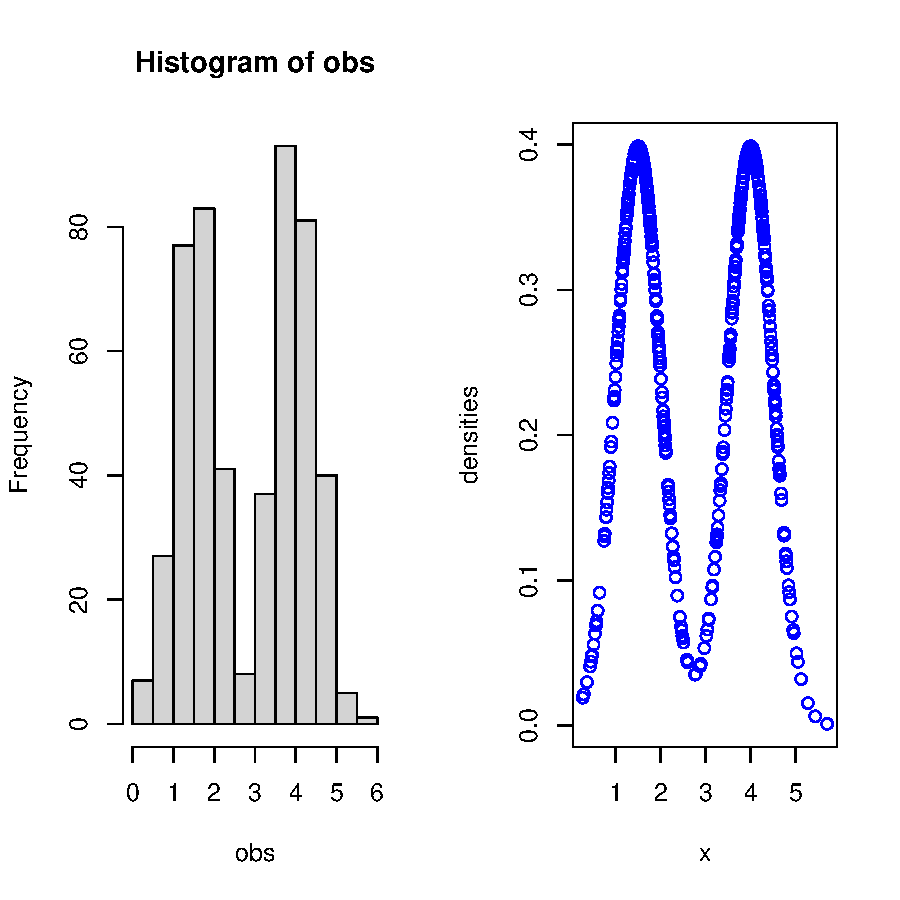
\includegraphics[width=\maxwidth]{figure/unnamed-chunk-27-1} 
\begin{kframe}\begin{alltt}
\hlkwd{par}\hlstd{(}\hlkwc{mfrow}\hlstd{=}\hlkwd{c}\hlstd{(}\hlnum{1}\hlstd{,}\hlnum{1}\hlstd{))}
\end{alltt}
\end{kframe}
\end{knitrout}


\subsection{3.7}
Now we implement a function that returns a vector of gamma values for each row in $\bm{X}$


\begin{knitrout}
\definecolor{shadecolor}{rgb}{0.969, 0.969, 0.969}\color{fgcolor}\begin{kframe}
\begin{alltt}
\hlstd{e_uni_two_comp} \hlkwb{<-} \hlkwa{function}\hlstd{(}\hlkwc{data}\hlstd{,} \hlkwc{theta}\hlstd{)\{}
  \hlstd{pi} \hlkwb{<-} \hlstd{theta}\hlopt{$}\hlstd{pi}
  \hlstd{mu1} \hlkwb{<-} \hlstd{theta}\hlopt{$}\hlstd{mu_1}
  \hlstd{mu2} \hlkwb{<-} \hlstd{theta}\hlopt{$}\hlstd{mu_2}
  \hlstd{sigma1} \hlkwb{<-} \hlstd{theta}\hlopt{$}\hlstd{sigma_1}
  \hlstd{sigma2} \hlkwb{<-} \hlstd{theta}\hlopt{$}\hlstd{sigma_2}
  \hlstd{numerator} \hlkwb{<-} \hlstd{pi}\hlopt{*}\hlkwd{dnorm}\hlstd{(data,} \hlkwc{mean}\hlstd{=mu2,} \hlkwc{sd}\hlstd{=sigma2)}
  \hlstd{denominator} \hlkwb{<-} \hlstd{(}\hlnum{1}\hlopt{-}\hlstd{pi)} \hlopt{*}\hlkwd{dnorm}\hlstd{(data,} \hlkwc{mean}\hlstd{=mu1,} \hlkwc{sd}\hlstd{=sigma1)} \hlopt{+} \hlstd{numerator}
  \hlstd{gamma_values} \hlkwb{<-} \hlstd{numerator} \hlopt{/} \hlstd{denominator}
  \hlkwd{return}\hlstd{(gamma_values)}
\hlstd{\}}

\hlstd{gamma} \hlkwb{<-} \hlkwd{e_uni_two_comp}\hlstd{(mixture_data, theta0)}
\hlkwd{t}\hlstd{(}\hlkwd{head}\hlstd{(gamma))}
\end{alltt}
\begin{verbatim}
          [,1]      [,2]      [,3]     [,4]      [,5]      [,6]
[1,] 0.9106339 0.8716861 0.7797225 0.664564 0.6484311 0.5178799
\end{verbatim}
\end{kframe}
\end{knitrout}

\subsection{3.8}
The gamma values are the irresponsibility for the observations. These responsibilities are obtained by the estimates of the parameters used in the function such that the responsibilities are assigned according to the relative density of the training under both models. For example, the first three obtained gamma values were 0.91, 0.87, and 0.78. These corresponds to the probabilities or weights that the first three observations belong to group 2 since component 2 is used as the base line component or so to speak .

\subsection{3.9}
Now we implement a function to return a list with the parameters given X and gamma.

\begin{knitrout}
\definecolor{shadecolor}{rgb}{0.969, 0.969, 0.969}\color{fgcolor}\begin{kframe}
\begin{alltt}
\hlstd{max_uni_two_comp} \hlkwb{<-} \hlkwa{function}\hlstd{(}\hlkwc{x}\hlstd{,} \hlkwc{gamma}\hlstd{)\{}
  \hlstd{mu_1} \hlkwb{<-} \hlkwd{sum}\hlstd{((}\hlnum{1}\hlopt{-}\hlstd{gamma)}\hlopt{*}\hlstd{x)} \hlopt{/} \hlkwd{sum}\hlstd{(}\hlnum{1}\hlopt{-}\hlstd{gamma)}
  \hlstd{mu_2} \hlkwb{<-} \hlkwd{sum}\hlstd{(gamma}\hlopt{*}\hlstd{x)} \hlopt{/} \hlkwd{sum}\hlstd{(gamma)}
  \hlstd{sigma_1_square} \hlkwb{<-} \hlkwd{sum} \hlstd{( (}\hlnum{1}\hlopt{-}\hlstd{gamma)} \hlopt{*} \hlstd{(x}\hlopt{-}\hlstd{mu_1)}\hlopt{^}\hlnum{2} \hlstd{)} \hlopt{/} \hlkwd{sum}\hlstd{(}\hlnum{1}\hlopt{-}\hlstd{gamma)}
  \hlstd{sigma_2_square} \hlkwb{<-} \hlkwd{sum}\hlstd{( gamma}\hlopt{*}\hlstd{(x}\hlopt{-}\hlstd{mu_2)}\hlopt{^}\hlnum{2} \hlstd{)} \hlopt{/} \hlkwd{sum}\hlstd{(gamma)}
  \hlstd{pi} \hlkwb{<-} \hlkwd{mean}\hlstd{(gamma)}

  \hlstd{results} \hlkwb{<-} \hlkwd{list}\hlstd{(}\hlstr{"mu_1"}\hlstd{= mu_1,} \hlstr{"mu_2"}\hlstd{=mu_2,} \hlstr{"sigma_1"}\hlstd{=} \hlkwd{sqrt}\hlstd{(sigma_1_square),}
                  \hlstr{"sigma_2"}\hlstd{=} \hlkwd{sqrt}\hlstd{(sigma_2_square),} \hlstr{"pi"}\hlstd{=pi)}
  \hlkwd{return}\hlstd{(results)}
\hlstd{\}}

\hlkwd{max_uni_two_comp}\hlstd{(mixture_data, gamma)}
\end{alltt}
\begin{verbatim}
$mu_1
[1] 3.842941

$mu_2
[1] 1.450413

$sigma_1
[1] 1.700666

$sigma_2
[1] 1.47168

$pi
[1] 0.4883709
\end{verbatim}
\end{kframe}
\end{knitrout}


\subsection{3.10}
Next we implement the log-likelihood as a function.

\begin{knitrout}
\definecolor{shadecolor}{rgb}{0.969, 0.969, 0.969}\color{fgcolor}\begin{kframe}
\begin{alltt}
\hlstd{ll_uni_two_comp} \hlkwb{<-} \hlkwa{function}\hlstd{(}\hlkwc{x}\hlstd{,} \hlkwc{theta}\hlstd{)\{}
  \hlstd{pi} \hlkwb{<-} \hlstd{theta}\hlopt{$}\hlstd{pi}
  \hlstd{mu1} \hlkwb{<-} \hlstd{theta}\hlopt{$}\hlstd{mu_1}
  \hlstd{mu2} \hlkwb{<-} \hlstd{theta}\hlopt{$}\hlstd{mu_2}
  \hlstd{sigma1} \hlkwb{<-} \hlstd{theta}\hlopt{$}\hlstd{sigma_1}
  \hlstd{sigma2} \hlkwb{<-} \hlstd{theta}\hlopt{$}\hlstd{sigma_2}
  \hlstd{log_lik} \hlkwb{<-} \hlkwd{log}\hlstd{((}\hlnum{1}\hlopt{-}\hlstd{pi)}\hlopt{*}\hlstd{(}\hlkwd{dnorm}\hlstd{(x,} \hlkwc{mean}\hlstd{=mu1,} \hlkwc{sd}\hlstd{=sigma1))} \hlopt{+}
                   \hlstd{pi}\hlopt{*}\hlkwd{dnorm}\hlstd{(x,} \hlkwc{mean}\hlstd{=mu2,} \hlkwc{sd}\hlstd{=sigma2))}
  \hlstd{total_sum} \hlkwb{<-} \hlkwd{sum}\hlstd{(log_lik)}
  \hlkwd{return}\hlstd{(total_sum)}
\hlstd{\}}
\hlkwd{ll_uni_two_comp}\hlstd{(mixture_data, theta0)}
\end{alltt}
\begin{verbatim}
[1] -43.1055
\end{verbatim}
\end{kframe}
\end{knitrout}

\subsection{3.11}
Now to combine the implemented function to an EM algorithm.


\begin{knitrout}
\definecolor{shadecolor}{rgb}{0.969, 0.969, 0.969}\color{fgcolor}\begin{kframe}
\begin{alltt}
\hlcom{#' @param X  n x P data matrix}
\hlstd{em_uni_two_comp} \hlkwb{<-} \hlkwa{function}\hlstd{(}\hlkwc{X}\hlstd{,} \hlkwc{theta0}\hlstd{,} \hlkwc{iter}\hlstd{)\{}
  \hlstd{gamma_matrix} \hlkwb{<-} \hlkwd{matrix}\hlstd{(}\hlnum{NA}\hlstd{,} \hlkwc{ncol}\hlstd{=}\hlkwd{nrow}\hlstd{(X),} \hlkwc{nrow}\hlstd{=iter)}
  \hlstd{theta_matrix} \hlkwb{<-} \hlkwd{matrix}\hlstd{(}\hlnum{NA}\hlstd{,} \hlkwc{ncol}\hlstd{=}\hlkwd{length}\hlstd{(theta0),} \hlkwc{nrow}\hlstd{=iter)}
  \hlstd{log_l_matrix} \hlkwb{<-} \hlkwd{matrix}\hlstd{(}\hlnum{NA}\hlstd{,} \hlkwc{ncol}\hlstd{=}\hlnum{1}\hlstd{,} \hlkwc{nrow}\hlstd{=iter)}
  \hlkwd{colnames}\hlstd{(theta_matrix)} \hlkwb{<-} \hlkwd{names}\hlstd{(theta0)}
  \hlcom{#initialize first theta}
   \hlstd{theta} \hlkwb{<-} \hlstd{theta0}
  \hlkwa{for} \hlstd{(i} \hlkwa{in} \hlnum{1}\hlopt{:}\hlstd{iter)\{}
    \hlstd{gamma_values} \hlkwb{<-} \hlkwd{e_uni_two_comp}\hlstd{(X, theta)}
    \hlstd{theta} \hlkwb{<-} \hlkwd{max_uni_two_comp}\hlstd{(X,} \hlkwc{gamma}\hlstd{=gamma_values)}
    \hlstd{l_lik} \hlkwb{<-} \hlkwd{ll_uni_two_comp}\hlstd{(}\hlkwc{x}\hlstd{=X,} \hlkwc{theta}\hlstd{=theta)}
    \hlstd{gamma_matrix[i,]} \hlkwb{<-} \hlstd{gamma_values}
    \hlstd{log_l_matrix[i,]} \hlkwb{<-} \hlstd{l_lik}
    \hlstd{theta_matrix[i,]} \hlkwb{<-} \hlkwd{do.call}\hlstd{(cbind, theta)}
    \hlkwd{cat}\hlstd{(}\hlstr{"Iter"}\hlstd{, i,} \hlstr{"Log Lik: "}\hlstd{,l_lik,} \hlkwc{fill} \hlstd{=} \hlnum{TRUE}\hlstd{)}

  \hlstd{\}}
   \hlkwd{return}\hlstd{(}\hlkwd{list}\hlstd{(}\hlstr{"gamma"} \hlstd{= gamma_matrix,} \hlstr{"log_l"}\hlstd{= log_l_matrix,} \hlstr{"theta"}\hlstd{= theta_matrix))}
\hlstd{\}}
\hlstd{em_res} \hlkwb{<-} \hlkwd{em_uni_two_comp}\hlstd{(mixture_data, theta0,} \hlkwc{iter} \hlstd{=} \hlnum{3}\hlstd{)}
\end{alltt}
\begin{verbatim}
Iter 1 Log Lik:  -41.53247
Iter 2 Log Lik:  -41.11211
Iter 3 Log Lik:  -40.48348
\end{verbatim}
\begin{alltt}
\hlstd{em_res}
\end{alltt}
\begin{verbatim}
$gamma
          [,1]      [,2]      [,3]      [,4]      [,5]      [,6]      [,7]
[1,] 0.9106339 0.8716861 0.7797225 0.6645640 0.6484311 0.5178799 0.2796799
[2,] 0.9178650 0.8894927 0.8167940 0.7116103 0.6955099 0.5528707 0.2519108
[3,] 0.9454468 0.9246043 0.8625704 0.7544583 0.7362906 0.5618554 0.1858035
           [,8]       [,9]      [,10]     [,11]     [,12]     [,13]     [,14]
[1,] 0.19920828 0.13010282 0.08432370 0.8769274 0.8361354 0.7700157 0.6627895
[2,] 0.15222465 0.07724154 0.03725366 0.8933796 0.8624511 0.8085676 0.7098561
[3,] 0.08785076 0.03210448 0.01096926 0.9275816 0.9028954 0.8548465 0.7524975
         [,15]     [,16]     [,17]      [,18]      [,19]       [,20]
[1,] 0.6411479 0.3606832 0.2202775 0.16169773 0.10099206 0.050519768
[2,] 0.6881296 0.3569185 0.1774257 0.10978815 0.05066204 0.015114749
[3,] 0.7278372 0.3091756 0.1103649 0.05404032 0.01723768 0.002916854

$log_l
          [,1]
[1,] -41.53247
[2,] -41.11211
[3,] -40.48348

$theta
         mu_1     mu_2  sigma_1  sigma_2        pi
[1,] 3.842941 1.450413 1.700666 1.471680 0.4883709
[2,] 3.967199 1.322309 1.641096 1.313247 0.4887533
[3,] 4.100188 1.179100 1.527945 1.145685 0.4880674
\end{verbatim}
\end{kframe}
\end{knitrout}



\subsection{3.12}
Now to test in on the mixture data for 20 iterations.
\begin{knitrout}
\definecolor{shadecolor}{rgb}{0.969, 0.969, 0.969}\color{fgcolor}\begin{kframe}
\begin{alltt}
\hlstd{em_res_20} \hlkwb{<-} \hlkwd{em_uni_two_comp}\hlstd{(mixture_data, theta0 ,} \hlkwc{iter} \hlstd{=} \hlnum{20}\hlstd{)}
\end{alltt}
\begin{verbatim}
Iter 1 Log Lik:  -41.53247
Iter 2 Log Lik:  -41.11211
Iter 3 Log Lik:  -40.48348
Iter 4 Log Lik:  -39.80459
Iter 5 Log Lik:  -39.3837
Iter 6 Log Lik:  -39.19062
Iter 7 Log Lik:  -39.07533
Iter 8 Log Lik:  -38.9989
Iter 9 Log Lik:  -38.95411
Iter 10 Log Lik:  -38.93147
Iter 11 Log Lik:  -38.92116
Iter 12 Log Lik:  -38.91669
Iter 13 Log Lik:  -38.91478
Iter 14 Log Lik:  -38.91397
Iter 15 Log Lik:  -38.91363
Iter 16 Log Lik:  -38.91348
Iter 17 Log Lik:  -38.91342
Iter 18 Log Lik:  -38.91339
Iter 19 Log Lik:  -38.91338
Iter 20 Log Lik:  -38.91338
\end{verbatim}
\begin{alltt}
\hlkwd{round}\hlstd{(em_res_20}\hlopt{$}\hlstd{theta[}\hlkwd{c}\hlstd{(}\hlnum{1}\hlstd{,}\hlnum{5}\hlstd{,}\hlnum{10}\hlstd{,}\hlnum{15}\hlstd{,}\hlnum{20}\hlstd{),],} \hlkwc{digits}\hlstd{=}\hlnum{3}\hlstd{)}
\end{alltt}
\begin{verbatim}
      mu_1  mu_2 sigma_1 sigma_2    pi
[1,] 3.843 1.450   1.701   1.472 0.488
[2,] 4.340 0.997   1.246   0.890 0.498
[3,] 4.609 1.051   0.948   0.875 0.544
[4,] 4.651 1.079   0.909   0.897 0.553
[5,] 4.655 1.083   0.905   0.900 0.554
\end{verbatim}
\end{kframe}
\end{knitrout}
The results for the parameters are pretty similiar, though they are not exactly equal for all decimals. Now we can plot the log-likelihood as well.

\begin{knitrout}
\definecolor{shadecolor}{rgb}{0.969, 0.969, 0.969}\color{fgcolor}\begin{kframe}
\begin{alltt}
\hlkwd{plot}\hlstd{(em_res_20}\hlopt{$}\hlstd{log_l,} \hlkwc{col}\hlstd{=}\hlstr{"green"}\hlstd{,} \hlkwc{type}\hlstd{=}\hlstr{"l"}\hlstd{,} \hlkwc{xlab}\hlstd{=}\hlstr{"Iteration"}\hlstd{,}
     \hlkwc{ylab}\hlstd{=}\hlstr{"Observed Data Log-likelihood"}\hlstd{)}
\hlkwd{points}\hlstd{(em_res_20}\hlopt{$}\hlstd{log_l,} \hlkwc{col}\hlstd{=}\hlstr{"green"}\hlstd{,} \hlkwc{pch}\hlstd{=}\hlnum{1}\hlstd{,} \hlkwc{cex}\hlstd{=}\hlnum{1.5}\hlstd{)}
\end{alltt}
\end{kframe}\begin{figure}
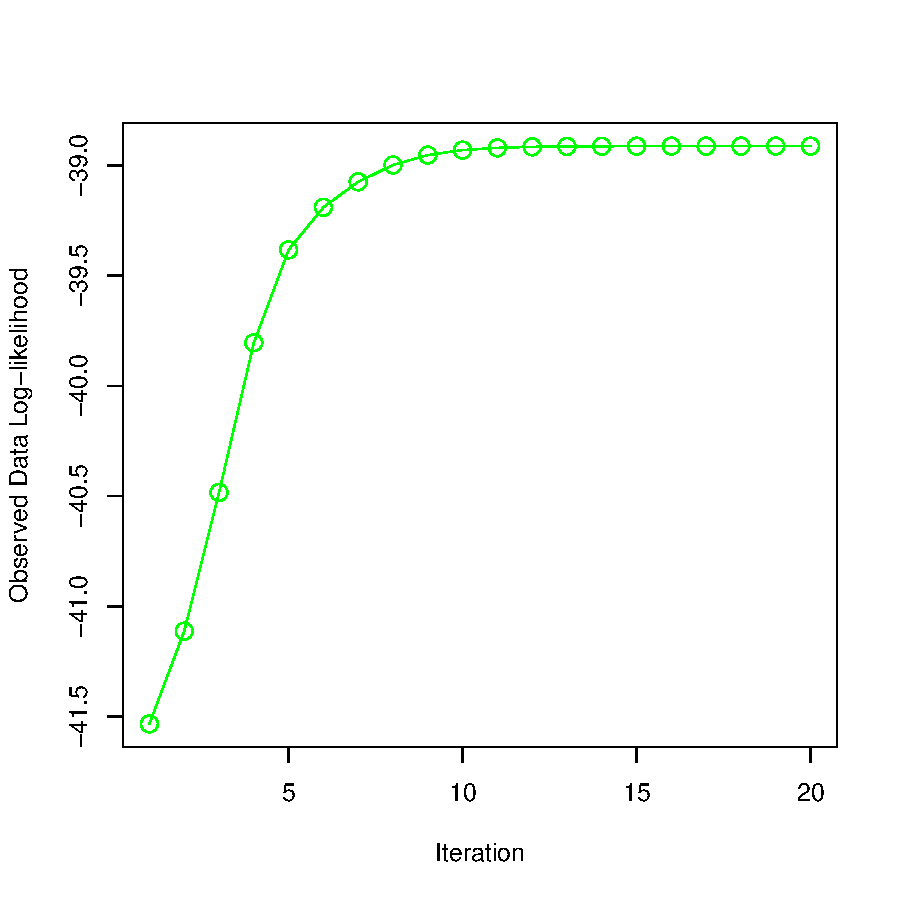
\includegraphics[width=\maxwidth]{figure/log_l_plot-1} \caption[EM algorithm]{EM algorithm: observed data log-likelihood as a function of the iteration number.}\label{fig:log_l_plot}
\end{figure}

\end{knitrout}

The plot is also pretty similar to the one in Hastie et al. 

\subsection{3.13}
Next we run the EM algorithm on the eruptions variable as well as Petal.Length.

\begin{knitrout}
\definecolor{shadecolor}{rgb}{0.969, 0.969, 0.969}\color{fgcolor}\begin{kframe}
\begin{alltt}
\hlstd{eruption_res} \hlkwb{<-}\hlkwd{em_uni_two_comp}\hlstd{(}\hlkwd{as.matrix}\hlstd{(faithful}\hlopt{$}\hlstd{eruptions), theta0 ,} \hlkwc{iter} \hlstd{=} \hlnum{20}\hlstd{)}
\end{alltt}
\begin{verbatim}
Iter 1 Log Lik:  -418.3729
Iter 2 Log Lik:  -416.5957
Iter 3 Log Lik:  -412.7431
Iter 4 Log Lik:  -402.6956
Iter 5 Log Lik:  -373.5664
Iter 6 Log Lik:  -320.9953
Iter 7 Log Lik:  -293.9944
Iter 8 Log Lik:  -280.3981
Iter 9 Log Lik:  -277.4294
Iter 10 Log Lik:  -276.816
Iter 11 Log Lik:  -276.567
Iter 12 Log Lik:  -276.4501
Iter 13 Log Lik:  -276.3969
Iter 14 Log Lik:  -276.3743
Iter 15 Log Lik:  -276.3654
Iter 16 Log Lik:  -276.362
Iter 17 Log Lik:  -276.3607
Iter 18 Log Lik:  -276.3603
Iter 19 Log Lik:  -276.3601
Iter 20 Log Lik:  -276.3601
\end{verbatim}
\begin{alltt}
\hlstd{petal_res}\hlkwb{<-} \hlkwd{em_uni_two_comp}\hlstd{(}\hlkwd{as.matrix}\hlstd{(iris}\hlopt{$}\hlstd{Petal.Length), theta0 ,} \hlkwc{iter} \hlstd{=} \hlnum{20}\hlstd{)}
\end{alltt}
\begin{verbatim}
Iter 1 Log Lik:  -293.4476
Iter 2 Log Lik:  -289.0347
Iter 3 Log Lik:  -277.2853
Iter 4 Log Lik:  -251.7706
Iter 5 Log Lik:  -217.0564
Iter 6 Log Lik:  -200.5795
Iter 7 Log Lik:  -200.5788
Iter 8 Log Lik:  -200.5788
Iter 9 Log Lik:  -200.5788
Iter 10 Log Lik:  -200.5788
Iter 11 Log Lik:  -200.5788
Iter 12 Log Lik:  -200.5788
Iter 13 Log Lik:  -200.5788
Iter 14 Log Lik:  -200.5788
Iter 15 Log Lik:  -200.5788
Iter 16 Log Lik:  -200.5788
Iter 17 Log Lik:  -200.5788
Iter 18 Log Lik:  -200.5788
Iter 19 Log Lik:  -200.5788
Iter 20 Log Lik:  -200.5788
\end{verbatim}
\begin{alltt}
\hlcom{#estimated parameters for iter 1,5,10,15, and 20}
\hlstd{eruption_res}\hlopt{$}\hlstd{theta[}\hlkwd{c}\hlstd{(}\hlnum{1}\hlstd{,}\hlnum{5}\hlstd{,}\hlnum{10}\hlstd{,}\hlnum{15}\hlstd{,}\hlnum{20}\hlstd{),]}
\end{alltt}
\begin{verbatim}
         mu_1     mu_2   sigma_1   sigma_2        pi
[1,] 3.825971 2.839693 1.0036998 1.1024940 0.3428935
[2,] 4.176372 2.396603 0.6629985 0.8462387 0.3868979
[3,] 4.285734 2.032232 0.4184247 0.2570452 0.3540938
[4,] 4.274590 2.019929 0.4351905 0.2377294 0.3489691
[5,] 4.273436 2.018705 0.4369244 0.2357767 0.3484463
\end{verbatim}
\begin{alltt}
\hlstd{petal_res}\hlopt{$}\hlstd{theta[}\hlkwd{c}\hlstd{(}\hlnum{1}\hlstd{,}\hlnum{5}\hlstd{,}\hlnum{10}\hlstd{,}\hlnum{15}\hlstd{,}\hlnum{20}\hlstd{),]}
\end{alltt}
\begin{verbatim}
         mu_1     mu_2   sigma_1   sigma_2        pi
[1,] 4.453807 2.358893 1.4580177 1.4540669 0.3321410
[2,] 4.924221 1.510104 0.8114996 0.3437946 0.3415879
[3,] 4.904976 1.461750 0.8232177 0.1716566 0.3331109
[4,] 4.904976 1.461750 0.8232177 0.1716566 0.3331109
[5,] 4.904976 1.461750 0.8232177 0.1716566 0.3331109
\end{verbatim}
\end{kframe}
\end{knitrout}
\subsection{3.14}
Lastly we visualize the densities for the two data sets using the parameters estimated with the EM-algorithm
\begin{knitrout}
\definecolor{shadecolor}{rgb}{0.969, 0.969, 0.969}\color{fgcolor}\begin{kframe}
\begin{alltt}
\hlcom{#Extracting thetas from last row of results}
\hlstd{eruption_theta} \hlkwb{<-} \hlstd{eruption_res}\hlopt{$}\hlstd{theta[}\hlkwd{nrow}\hlstd{(eruption_res}\hlopt{$}\hlstd{theta),]}
\hlcom{#converting thetas to list}
\hlstd{eruption_theta_list} \hlkwb{<-} \hlkwd{list}\hlstd{()}
\hlkwa{for}\hlstd{(i} \hlkwa{in} \hlnum{1}\hlopt{:}\hlnum{5}\hlstd{)\{}
  \hlstd{eruption_theta_list[[}\hlkwd{names}\hlstd{(eruption_theta)[i]]]} \hlkwb{<-} \hlstd{eruption_theta[i]}
\hlstd{\}}

\hlkwd{par}\hlstd{(}\hlkwc{mfrow}\hlstd{=}\hlkwd{c}\hlstd{(}\hlnum{1}\hlstd{,}\hlnum{2}\hlstd{))}
\hlkwd{hist}\hlstd{(faithful}\hlopt{$}\hlstd{eruptions)}
\hlkwd{plot_density}\hlstd{(}\hlkwc{x}\hlstd{=faithful}\hlopt{$}\hlstd{eruptions,} \hlkwc{theta}\hlstd{=eruption_theta_list,}
             \hlkwc{main}\hlstd{=}\hlstr{"Densities for Eruption data"}\hlstd{)}
\end{alltt}
\end{kframe}\begin{figure}
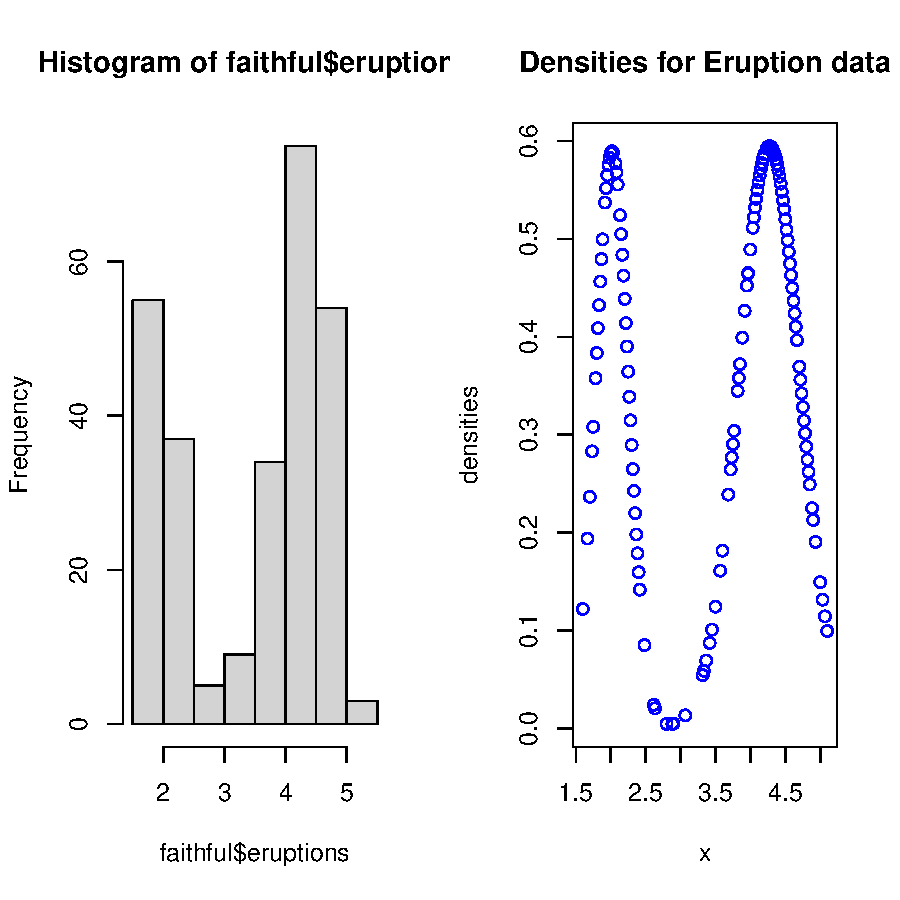
\includegraphics[width=\maxwidth]{figure/unnamed-chunk-34-1} \caption[Densities for eruptions]{Densities for eruptions}\label{fig:unnamed-chunk-34}
\end{figure}

\end{knitrout}

\begin{knitrout}
\definecolor{shadecolor}{rgb}{0.969, 0.969, 0.969}\color{fgcolor}\begin{kframe}
\begin{alltt}
\hlstd{petal_theta} \hlkwb{<-} \hlstd{petal_res}\hlopt{$}\hlstd{theta[}\hlkwd{nrow}\hlstd{(petal_res}\hlopt{$}\hlstd{theta),]}
\hlstd{petal_theta_list} \hlkwb{<-} \hlkwd{list}\hlstd{()}
\hlkwa{for}\hlstd{(i} \hlkwa{in} \hlnum{1}\hlopt{:}\hlnum{5}\hlstd{)\{}
  \hlstd{petal_theta_list[[}\hlkwd{names}\hlstd{(petal_theta)[i]]]} \hlkwb{<-} \hlstd{petal_theta[i]}
\hlstd{\}}
\hlkwd{par}\hlstd{(}\hlkwc{mfrow}\hlstd{=}\hlkwd{c}\hlstd{(}\hlnum{1}\hlstd{,}\hlnum{2}\hlstd{))}
\hlkwd{hist}\hlstd{(iris}\hlopt{$}\hlstd{Petal.Length)}
\hlkwd{plot_density}\hlstd{(}\hlkwc{x}\hlstd{=iris}\hlopt{$}\hlstd{Petal.Length,} \hlkwc{theta}\hlstd{=petal_theta_list,}
             \hlkwc{main}\hlstd{=}\hlstr{"Densities for Petal length data"}\hlstd{)}
\end{alltt}
\end{kframe}\begin{figure}
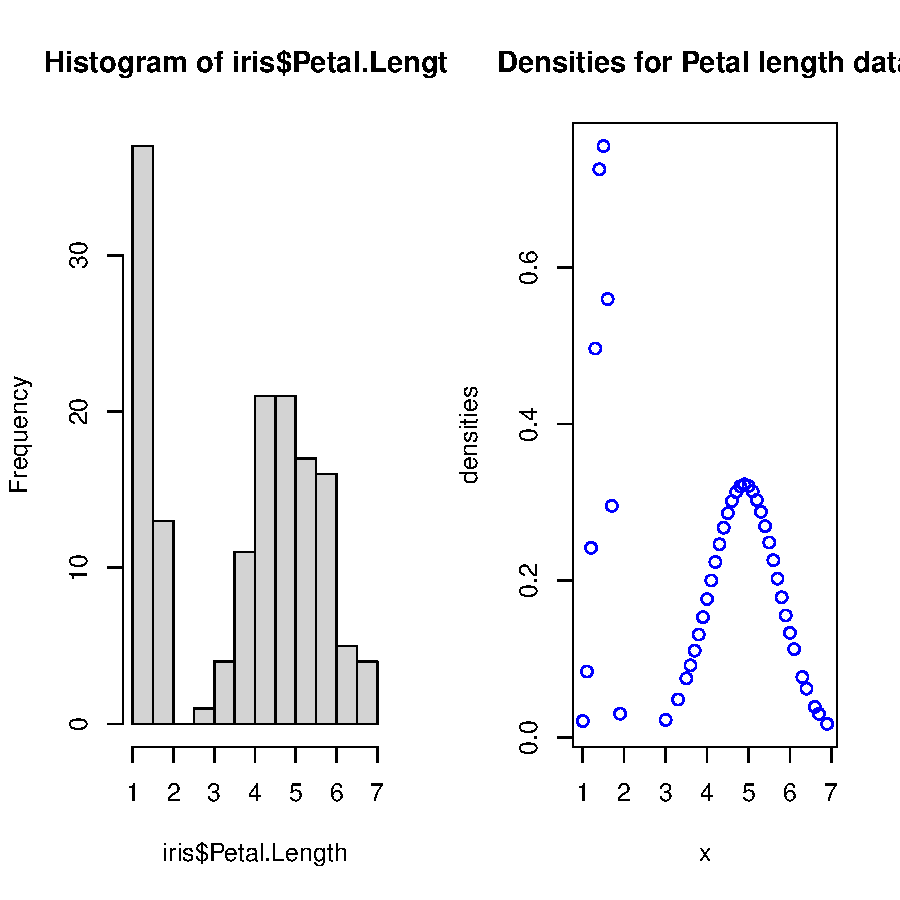
\includegraphics[width=\maxwidth]{figure/unnamed-chunk-35-1} \caption[densities for petal length]{densities for petal length}\label{fig:unnamed-chunk-35}
\end{figure}

\end{knitrout}

\end{document}
